%%%%%
%This is the main file.  This is where you set up your preferences, name the packages you need, and use the "input" command to order the chapters and other major components of your thesis, most of which are set up as separate .tex files.  To see other project files, click the "Project" tab on the upper left.  If you click on a section in the pdf preview, you will jump to that file (Overleaf).
%%%%%

\documentclass[12pt]{report}  %12 point font is set - Times New Roman is the default

%These are a bunch of packages that may or may not be needed for features I use later
\usepackage{graphicx}
\usepackage{caption}                     % For captions
\usepackage{subcaption}
\usepackage{float}                       % For [H] placement
\usepackage[table]{xcolor}
\usepackage{amsmath}
\usepackage{hyperref}
\usepackage{url}
\usepackage{multicol}
\usepackage{booktabs}
\usepackage[toc,page]{appendix}
\usepackage{glossaries}
\makenoidxglossaries

\newacronym{cdr}{CDR}{Creighton Digital Repository}
\newacronym{icrp}{ICRP}{International Commission on Radiological Protection}
\newacronym{eerd}{EERD}{entrance exposure rate to detector}
\newacronym{seer}{SEER}{skin entrance exposure rate}
\newacronym{xrii}{XRII}{image intensifier}
\newacronym{ir}{IR} {interventional radiology}
\newacronym{snr}{SNR} {signal-to-noise ratio}
\newacronym{aapm}{AAPM} {American Association of Physicists in Medicine}
\newacronym{cumc}{CUMC}{Creighton University Medical Center}
\newacronym{bmmc}{BMMC}{Bergan Mercy Medical Center}
\newacronym{lnt}{LNT}{linear no-threshold}
\newacronym{rfl}{rad/fluoro}{radiography/fluoroscopy}
\newacronym{alara}{ALARA}{``as low as reasonably achievable"}

\newacronym{aerc}{AERC}{automatic exposure rate control}

\newacronym{dap}{DAP}{dose area product}

\newacronym{tld}{TLD} {thermoluminescent dosimeter}

\newacronym{dis}{DIS}{direct ion storage}

\newacronym{ic}{IC}{ion chamber}

\newacronym{sid}{SID}{source-to-image distance}

\newacronym{ssd}{SSD}{source-to-surface distance}
\newacronym{ecg}{ECG}{electro cardigram}
\newacronym{rf}{RF}{radiofrequency}

\newacronym{cied}{CIED}{cardiac implantable electronic device}
\newacronym{hrs}{HRS}{Heart Rhythm Society}

\newacronym{pd}{PD}{Proton Density}
\newacronym{pla}{PLA}{Polylactic Acid}
\newacronym{pvc}{PVC}{Polyvinyl Chloride}


\newacronym{mosfet}{MOSFET}{metal-oxide-semiconductor field-effect transistor}
\newacronym{mri}{MRI}{Magnetic Resonance Imaging}

\newacronym{nvlap}{NVLAP}{National Voluntary Lab Accreditation Program}

\newacronym{epd}{EPD}{electronic personal dosimeter}

\definecolor{steelblue}{rgb}{0.27, 0.51, 0.71}
\definecolor{crimson}{rgb}{0.86, 0.08, 0.24}
\definecolor{darkslategray}{rgb}{0.18, 0.31, 0.31}

\hypersetup{colorlinks   = true, %Colours links instead of ugly boxes
	urlcolor     = steelblue, %Colour for external hyperlinks
	linkcolor    = darkslategray, %Colour of internal links
	citecolor   = crimson %Colour of citations
    }
\renewcommand\bibname{References}
\usepackage{setspace}
\usepackage[letterpaper,left=1.5in,right=1in,top=1in,bottom=1in]{geometry} %margin of bound side 1.5 in, rest of margins 1 in, per Creighton Thesis guideline formats

\usepackage{draftwatermark}
\usepackage{tikz}
\usetikzlibrary{shapes.geometric, arrows,positioning}

\tikzstyle{startstop} = [rectangle, rounded corners, minimum width=3cm, minimum height=1cm,text centered, draw=black, fill=red!20]
\tikzstyle{process} = [rectangle, minimum width=3cm, minimum height=1cm, text centered, draw=black, fill=blue!20]
\tikzstyle{decision} = [diamond, minimum width=3cm, minimum height=1cm, text centered, draw=black, fill=green!20, aspect=2]
\tikzstyle{arrow} = [thick,->,>=stealth]

\usepackage{pdfpages}                    % For appendix PDFs
\usepackage{pdflscape}
%\usepackage{subfigure}
\usepackage{pdfpages}
\widowpenalty10000% This automatically groups lines so there is at least 2 from each paragraph on a page.  Optional
\clubpenalty10000 %see above comment
\usepackage{indentfirst} %This makes the first paragraph of a section indented.  Optional.
\usepackage{breqn}
\usepackage[en-US]{datetime2}

\begin{document}

\newpage
\thispagestyle{empty}
\mbox{}
\clearpage %blank page at beginning of pdf.  not numbered

\begin{titlepage}

	\begin{center}

		THESIS APPROVED BY\\
		\vspace{1.5cm}
    \end{center}
		\line(1,0){200} \hspace{2cm} \line(1,0){200} \\	
		Date \hspace{8cm} [Michael Nichols], Ph.D.
		\vspace{1.5cm}\\
        \null \hspace{9cm} \line(1,0){200} \\	
		\null \hspace{9cm} [Hill], Ph.D.
        \vspace{1.5cm}\\
		\null \hspace{9cm} \line(1,0){200} \\	
		\null \hspace{9cm} [Wrubel], Ph.D.
        \vspace{2.5cm}\\
		\null \hspace{9cm} \line(1,0){200} \\	
		\null \hspace{9cm} Gail M. Jensen, Ph.D., Dean
%% Print out as many copies of this page as you will be making bound copies.   Then, have all your committee members sign the page and give to the grad office.  Dr. Jensen will sign them and Taunya will hang onto them for insertion into the bound copies.  They will email you a pdf copy which you will insert into the digital copy of the thesis.  Remember to delete the blank signature page!  	
	

\end{titlepage} %Have this page printed and signed, then delete from your thesis and insert the signed version.

%\includepdf[scale=1.0]{Sig2.pdf} % After the dean signs the approval page, LuAnn Schwery sends you a pdf, which you insert into your thesis

\pagenumbering{roman} %begin roman numeral page numbers for the front matter


	\begin{center}
		{\LARGE \scshape{Title: \\\large Subtitle}} % you can format this how you like, but it is usually in all-caps
		
		
		\vspace{4cm}
		\line(1,0){200} \\
		\vspace*{0.5cm}
		by \\	
		\vspace*{0.5cm}
		\large \scshape{
		Daniel Juarez Luna}
		\vspace*{0.5cm}
		
		\line(1,0){200}
		
		\vspace{3cm}
		\textsc{
		A Thesis }

		
		\vspace{2cm}
	\textnormal{	Submitted to the faculty of the Graduate School of Creighton University in Partial
Fulfillment of the Requirements for the degree of Master of Science in [Physics/Medical Physics] (choose one) in the Department of Physics}
		
		\vspace{1cm}
		\line(1,0){200} \\	
		\vspace*{1cm}	\textnormal{
		Omaha, NE\\
		\today}
	\thispagestyle{empty}
	\end{center}
 %title page

\doublespacing

\SetWatermarkText{DRAFT}
\SetWatermarkScale{3}
\SetWatermarkLightness{0.85}
\SetWatermarkAngle{45}

\newpage %insert blank page, counted in page numbers
\thispagestyle{empty} % do not display page number
\mbox{}
\clearpage 

\addcontentsline{toc}{chapter}{Abstract} %include abstract in table of contexts.  Chicago Manual of Style argues against having any front matter before the TOC included in the TOC


\chapter*{Abstract}

The abstract is a maximum 350 word, double-spaced summary of your work.  The word count limit is important for upload to the Creighton Digital Repository.

This project can be found as a template on the Overleaf.com Latex-writing website.  %Abstract is the first thing in the thesis after the title

\clearpage

\addcontentsline{toc}{chapter}{Acknowledgments}  %includes abstract in table of contexts.  Chicago Manual of Style argues against listing front matter that is before the TOC in the TOC


\chapter*{Acknowledgments} 

Thank your research team, advisor, committee, family and friends, etc.  See previous theses for examples.

I would like to thank Kian for introducing me to Latex, Kyle and Bong for troubleshooting help, and Dr. Nichols for his help with thesis creation.


 %optional

\clearpage

\addcontentsline{toc}{chapter}{Dedication}%includes dedication in table of contexts.  Chicago Manual of Style argues against listing front matter that is before the TOC in the TOC


%no page number on dedication page

\thispagestyle{empty}
\begin{normalsize}
\vspace*{\fill}
\begingroup
\centering
\begin{center}
	\textit{For Dr. Nichols} %Optional page
\end{center}
\endgroup
\vspace*{\fill}
\end{normalsize}

 %optional

\clearpage


\tableofcontents %automatically generate TOC
\clearpage

\listoftables %automatically generates list of tables
\clearpage
\listoffigures%automatically generates list of figures

\clearpage


\pagenumbering{arabic} % start normal numbering on the first page of chapter 1

%\input{chapter1}



%Establishing Context and Problem Statement
%state briefly and clearly your purpose in writing the paper
%the nature and scope of the problem investigated, indicating why the overall subject area is important

%"funnel" shape


%"contextualizing background,"
%For knowledgeable peers, a quick opening is appropriate, implying familiarity with the concepts. For less technical or less informed audiences, a slower, more patient explanation of concepts may be necessary


%explicitly state the "statement of the problem," which includes a condition of incomplete knowledge or understanding, and the significant consequences or costs of that condition if it remains unresolved, or the benefits if it is solved (the "So what?" question)


%Literature Review: is a literature review valuable?

% briefly review the pertinent literature to orient the reader and identify the gap in the existing literature that the current research aims to address

%summarize only the key points from sources most relevant to your argument, especially those you intend to challenge, modify, or expand upon


%Objective and Method: The introduction should then make clear the objective of the research.  state the method of the investigation, and, if necessary, briefly explain the reasons for choosing a particular method


%Results and Conclusions (Optional): end by stating the principal results. promise a solution or main point that will be revealed later in the paper


\chapter {Introduction}

%Why is the overall subject area of your research important?.
Medical diagnostics heavily rely on imaging tools such as \gls{mri}, a powerful and evolving application capable of showing high contrast sensitivity to soft tissue while not depending on ionizing radiation. However, safety concerns may arise during cardiac MRI procedures, \gls{ecg} leads are generally cataloged as  \gls{mri} unsafe because of the strong magnetic field and \gls{rf} pulses that may interact with these leads.

Temporary epicardial pacing leads are frequently utilized as part of postoperative cardiac rhythm control procedures. When the surgical danger of removing these leads is too high, they are left in place to prevent further complications. These cases introduce long-term repercussions, most notably the loss of access to \gls{mri}. There is still a dearth of focused studies evaluating the precise dangers associated with retained epicardial leads, despite the frequent use of such leads and their repercussions. Existing clinical recommendations tend to be too cautious and frequently disqualify these individuals from \gls{mri} eligibility even when there is little evidence to support it.


%outline the thesis
In this document we will explain the current state of research on this matter, the main elements involved in the interaction of temporary epicardial leads and \gls{mri} - especially in relation to mechanical interactions like translational force and torque. We will explore... and propose a methodology that tests these micro-Newton forces with precision 


%What are the significant consequences or costs of this condition if it remains unresolved, or the benefits if it is solved (the "So what?" question)?. How will not knowing the answer to your research question keep your readers from understanding something else more important?.

More than 300,000 individuals are receiving new \gls{cied} implants every year in the U.S. alone, reported the \gls{hrs} in 2024 \cite{HRS2024_CIEDs}. Some of these patients will eventually require device explantation or revision, necessitating surgery \cite{Mubarak:2023aa}. For this, there is a protocol to monitor cardiac rhythm that involves the use of temporary epicardial leads, however there is a recognized practice when these leads are removed -only if significant resistance is encountered- to cut the wire flush with the skin, intentionally leaving a small segment inside the patient to prevent immediate complications \cite{aboyewa2021, doi:10.2214/ajr.168.5.9129404,PSA_Advisory_2006}.

These provisional leads are frequently placed during open-heart surgery to regulate cardiac rhythm postoperatively, then are typically cut at the skin surface leaving behind a short length of wire embedded in the tissue \cite{reade2007}. In general, a device labeled as MRI safe is expected to be nonconductive, non-electrical, non-magnetic, and to present no known hazards in the MRI environment. However, this classification does not apply to most epicardial leads, as they are rarely physically characterized after removal. By the time they are cut, these leads have fulfilled their clinical purpose, and systematic safety evaluations are seldom performed. Although retained leads are nonfunctional and relatively short, they are frequently classified as MRI unsafe due to concerns over \gls{rf} heating, magnetically induced translational forces and torques, or inadvertent cardiac stimulation \cite{poh2017,muthalaly2018,ACC_2024_MRI_CIEDs}. Effectively preventing patients with \gls{cied} or cardiac surgery history, who are most likely to need a \gls{mri} scan during their lifetime, to not be able to enter \gls{mri} room. 

Recent studies regarding this problem have shown both no image quality degradation and, most importantly, no serious safety events such as, device malfunction, myocardial injury or arrhythmias, associated with \gls{mri} examinations in patients with \gls{cied}s abandoned leads, including epicardial leads \cite{vuorinen2021,meier2024}. While these work have evaluated to some extent the resulting consequences of \gls{rf}-induced heating, mechanical forces and conductivity, detail is needed. For example translational motion and torque remain physically under-characterized.

%What specific condition of incomplete knowledge or understanding does your research address within this context?.

In that regard, the primary safety concerns regarding retained cardiac leads during \gls{mri} arise from three main interaction mechanisms. First, the strong magnetic field and its spatial gradient can exert translational forces and torques on the lead, resulting in mechanical displacement. Second, the lead can absorb energy from the \gls{mri}’s (\gls{rf}) field, potentially causing localized heating that poses a thermal risk to the patient. Third, the \gls{rf} field may induce alternating currents within the lead, which can electrically stimulate nearby cardiac tissue, potentially leading to dangerous physiological effects.
 
 To properly situate this work, the following section will review pertinent literature on \gls{mri} devices, \gls{mri} safety principles, electromagnetic theory, lead design, lead-\gls{mri} interactions and previous studies to establish the technical and clinical context needed to fully understand the motivations and significance of this study.

\section{Literature review}


%What is the "stable context" or general understanding that your research will challenge or build upon?.

%Epicardial leads design
%Types
%Uses


%materials employed


%sizes

%how this tech have evolved making it safer on the medical settings
%current state of the institutions that recommend saferty around MRI
%Which leads are we testing on? Why this leads in particular? %todo


\subsection{\gls{mri}: How it works?}

% ------------------------------------------------------------------------------
% MRI Translational Forces – Background Section Writing Guide
%
% Section Structure with Topic Priorities:
%
% 1. Introduction
%    - What is MRI and why is it used clinically      [🟠 Medium Priority]
%      (Keep brief—serves as justification for MRI relevance to clinical care.)
%
% 2. Magnetic Interactions
%    - Magnetic Moments & Magnetization              [🔴 High Priority]
%      (Foundation for understanding how magnetic fields act on materials.)
%    - Material Susceptibility (Δχ)                  [🔴 High Priority]
%      (Include MR compatibility thresholds—Δχ < 0.01 for safety.)
%
% 3. MRI System Components
%    - Main Magnet                                   [🔴 High Priority]
%      (Primary source of static magnetic field and spatial gradients.)
%    - Gradient Coils                                [🟠 Medium Priority]
%      (Include brief note on eddy currents and induced Lorentz forces.)
%    - RF Coils (Antennas)                           [🟡 Low Priority]
%      (Mention briefly if relevant to antenna effect in retained leads.)
%
% 4. Background Physics
%    - Resonance & Larmor Frequency                  [🟠 Medium Priority]
%      (Describe precession, gyromagnetic ratio; sets up how B₀ interacts with protons.)
%    - T1/T2 Relaxation                              [🟡 Low Priority]
%      (Tissue-level effects, not directly tied to mechanical forces; keep concise.)
%
% 5. Out of Scope (Omit or Defer to Appendix)
%    - Signal Localization and K-Space               [⚪ Skip]
%    - Image Acquisition Parameters & Weighting      [⚪ Skip]
%    - Basic Pulse Sequences                         [⚪ Skip]
%
% Legend:
%   🔴 High Priority   – Discuss in full detail
%   🟠 Medium Priority – Cover briefly, emphasize relevance
%   🟡 Low Priority    – One or two sentences max
%   ⚪ Skip            – Omit unless contextually needed
% ------------------------------------------------------------------------------


%	Quick review on the MRI components and principles


% 1. Introduction
%    - What is MRI and why is it used clinically      [🟠 Medium Priority]
\gls{mri} or Magnetic Resonance Imaging is a medical imaging modality that uses magnetic fields and radiofrequency (\gls{rf}) energy to produce images, rather than ionizing radiation like X-rays making it inherent safe. \gls{mri} machines are capable of archiving high contrast sensitivity to soft tissue differences because of the reliance on micromagnetic properties of the tissue and its inherent differences leveraging on \gls{pd} and the relaxation phenomena.



% 2. Magnetic Interactions
%    - Magnetic Moments & Magnetization              [🔴 High Priority]
%      (Foundation for understanding how magnetic fields act on materials.)
%    - Material Susceptibility (Δχ)                  [🔴 High Priority]
%      (Include MR compatibility thresholds—Δχ < 0.01 for safety.)


forces are described as a function of the static field strength ($B_0$), its spatial gradient ($\nabla B_0$), and the magnetic susceptibility ($\chi$) and density ($\rho$) of the material. A well known and expected behavior is the magnetic pull on high susceptibility materials toward regions of higher field strength, like near the bore entrance of the scanner where the spatial gradient is highest \cite{aboyewa2021,bushberg2011,panych2018}. For instance, a nonmagnetic stainless steel wire with $\chi \approx 103$ ppm may experience a force equivalent to $\sim$30\% of its weight, whereas ferromagnetic materials like pure nickel can experience forces exceeding 20,000 times their own weight. That is more than enough to become dangerous projectiles unless restrained \cite{aboyewa2021,panych2018}.

\subsubsection{Components:}

% 3. MRI System Components
%    - Main Magnet                                   [🔴 High Priority]
%      (Primary source of static magnetic field and spatial gradients.)
%    - Gradient Coils                                [🟠 Medium Priority]
%      (Include brief note on eddy currents and induced Lorentz forces.)
%    - RF Coils (Antennas)                           [🟡 Low Priority]
%      (Mention briefly if relevant to antenna effect in retained leads.)

For heat and electricity we are particularly interested on RF fields
for mechanical we need to know the static magnetic field
the mechanisim and intesity of the field

Now we can explain the interactions between the two. Once RF is understood we can explain how this affect the leads resulting in heating and electric conductivity, based on the past local research and literature.			



%//////////
the physics

Resonance and Signal Generation


Tissue Contrast (Relaxation Phenomena)

the interaction
%//////////

\subsection{Safety}

the safety
the 5 gauss line
the examples of safety
ASTM translational and torques studies
the current protocols to assess objects near MRI field
how this is different for us, size and suceptibility



ASTM F2052-21 offers a standardized technique for assessing magnetically induced displacement force on medical equipment in order to set safety standards for such situations. This standard states that a device is MR Conditional if the deflection force it encounters in the MRI environment is less than the force of gravity upon it. This is usually verified if the deflection angle from vertical is less than 45$^\circ$ \cite{stoianovici2024,astmF2052}.
 %halfway there

\subsection{Instruments?}

Gaussmeter and Hall effect?

\subsection{Previous studies summary}
%What pertinent literature needs to be reviewed to orient the reader and provide sufficient background information for them to understand your study?.

%What are the main arguments or findings from the sources most relevant to your argument, especially those you intend to challenge, modify, or expand upon?.

%Have there been previous effective reviews of your subject, and if so, what is the starting point (e.g., date of previous review) for your current review?.
Previous studies made in our institution seek to illustrate the interaction of leads with the \gls{rf} field in terms of energy absorbed and heat produced. It showed that lead length, type, and orientation significantly influence heating behavior.This study found that short leads ($<13$ cm) posed no significant thermal hazard during MRI at a specific absorption rate (SAR) of 2 W/kg and is throughtfully described as Master Thesis in 2021 \cite{haddixProposal,astmF2182,aboyewa2021}.

Along the same line of thought, we aim to cover the mechanical aspect of lead-\gls{mri} interaction covering (1) Characterization of the static magnetic field, (2) quantification of translational forces near the bore entrance, (3) Torque evaluation from bore entrance to isocenter.

While some preliminary work has been conducted in our lab on these mechanical concerns, it remains unpublished, making this thesis a critical step in formalizing and extending that foundational effort.


\section{Scope of Research}

From here onwards I only stated the answers to some common questions the intro addresses.

What is the nature and scope of the problem you investigated?.

This research addresses the safety implications of retained temporary epicardial pacing leads during MRI procedures. Although these leads are commonly left in place after cardiac surgeries to avoid surgical risks, their presence is often treated as a contraindication for MRI access due to theoretical concerns over RF-induced heating, induced currents, and mechanical forces. While some studies have begun to evaluate heating and image quality, the mechanical interactions—specifically translational forces and torque—remain undercharacterized. This thesis focuses on quantifying those mechanical forces in order to clarify whether the static magnetic field in MRI poses a real risk to patients with retained leads.



What is the clear objective of your research?.

The primary objective of this study is to experimentally characterize the translational magnetic forces acting on retained epicardial pacing leads near the MRI bore entrance, and to map how those forces evolve with distance from the isocenter. This aims to directly assess whether the magnitude of such forces constitutes a meaningful mechanical risk in clinical settings.



What's the specific hypotheses or research questions that your study addressed?.

The central research question is: Do retained epicardial pacing leads experience translational magnetic forces within an MRI environment that are clinically significant enough to justify current safety restrictions?



What is your purpose in writing this paper?

The purpose of this thesis is to provide experimental evidence on MRI-induced mechanical forces acting on retained cardiac leads, with the goal of informing clinical decision-making regarding MRI safety. By addressing a gap in the literature, the study seeks to support more nuanced guidelines that balance patient safety with access to essential imaging.


What method of investigation did you use in your study?.

In the lab, the investigation used a PVC controlled pendulum-based measurement setup simulating exposure to a magnetic field gradient similar to that found at the MRI bore entrance. A solenoid coil was employed to replicate the spatial gradient of the static magnetic field, and micro-Newton displacements were recorded to estimate translational forces on test rods. For torque a set of neodymium magnets would create the static field while a metallic rod would be fixed in a position perpendicular to the field with an attachment and be allowed to rotate, counter forces would then be measured out the attachment with a circuit and sensor of our own fabrication.


What were the reasons for choosing your particular method?.

These methods allow for high sensitivity in detecting small magnetic forces in a controlled environment, without the complications of patient variability or direct MRI scanner use. The pendulum approach provides a clear physical model that isolates translational force components for precise characterization. The torque model allows to independently assess strength of force exerted.



Materials and methods bridge [placeholder]

What are the few key concepts and themes that will run through all parts of your thesis, starting from this introduction?

The thesis will consistently engage with 1 of the 3 main interaction modes between MRI and retained leads: mechanical forces, RF-induced heating, and induced currents. In these mechanical forces aspect we particularly care about translational and rotational displacement due to static field gradients. Concepts from electromagnetism, MRI safety standards, and biomedical device regulation form the thematic backbone of the work.

Measurements are interpreted in the context of magnetic susceptibility theory and compared to relevant thresholds from the literature \cite{haddixProposal,astmF2052}. These techniques will help with more thorough evaluations of MRI safety in patients with retained temporary epicardial leads and set the stage for a future clinical adaptation of the protocol employing a 1.5 T MRI scanner. This method aids in the improvement of device classification and the creation of uniform experimental procedures for the assessment of torque and translational safety.



%\input{chapter2}
\chapter {Materials and Methods}

The objective of this study was to measure and quantify MRI-induce translational and torque forces experienced by an  post-surgical epicardial pacing leads when exposed to the static magnetic field. Safety limits for MRI magnetic fields are well established and described in the Introduction, based on ASTM F-series guidelines. Following these methods, we constructed non-magnetic test apparatus specifically designed to measure these forces with the precision required for clinical applications.

However, clinical access for experimental testing posed a significant challenge, as MRI scanner time is typically associated with long scheduling delays and short available measurement periods. Therefore, a secondary objective of this work was to improve the quality of our experimental setup in order to maximize the efficiency of data acquisition during these limited observation windows.

Previous students developed the laboratory-scale instruments and associated software necessary to evaluate magnetic forces in a controlled environment. This was achieved by generating a smaller but reproducible magnetic field in the laboratory, enabling characterization of materials with relatively high magnetic susceptibility. While this laboratory-generated field was not sufficient to directly measure or characterize the epicardial lead itself, it allowed for evaluation of the accuracy and measurement capacity of each instrument, as well as for the observation of the physical phenomena described above. Furthermore, given the proportional nature of the magnetic effects on a material, it was expected that, when tested in the much stronger (3 T) magnetic field of a clinical MRI system, the small magnetic susceptibility of the epicardial lead would not present a significant limitation in terms of measurement accuracy.

Three distinct experimental setups were involved in this study: (1) a spatial field mapping platform to characterize $B_0$ and $\nabla B_0$, (2) a pendulum-based deflection apparatus to assess translational force through angular displacement, and (3) a torque measurement system for rotational force assessments. In this chapter we will explain our setup and rationale, as well as the proven modifications to the instruments in order to provide a reproducible map of action to test our instruments.

\subsection*{Magnetic Field Generation}

Magnetic fields were generated using a \textbf{custom-built air-core solenoid}, approximately 15 cm in length and 10 cm in outer diameter. The solenoid was densely wound with \textbf{copper wire ($\sim$1 mm diameter)}, forming an inner core of approximately 5 cm. A \textbf{Pasco Scientific SF-9584 DC power supply} was used to deliver currents in the range of \textbf{0--4 A}, corresponding to magnetic field strengths from \textbf{1 to 18.9 Gauss} for this solenoid. The system operated in a continuous mode; no rest periods were applied between trials due to the time required to stabilize the pendulum after each adjustment. 

\subsection{Magnetic Field and Gradient Mapping Platform}

Magnetic field strength ($B_0$) and gradient ($\nabla B_0$) measurements were performed using a commercial Gaussmeter (Model GM2, AlphaLab Inc., Salt Lake City, UT).  The GM2 operates on the Hall effect principle, wherein a voltage is generated across a probe when exposed to a perpendicular magnetic field. This voltage is proportional to the local magnetic flux density, enabling precise spot measurements of field magnitude. The Gaussmeter used has an accuracy of 1\% of the DC reading in the 16$^\circ$C to 29$^\circ$C range.

To ensure spatial accuracy and reproducibility, a fixture made from rigid \gls{pvc} was constructed by previous Creighton University students \cite{haddixProposal}. The platform comprises a 300 mm square base and a 280 mm diameter vertical circular plate, perforated with a 5x5 grid of probe-access holes spaced at 20 mm intervals as shown in figure \ref{fig:fieldmapping}. Each access point was numerically indexed to facilitate 2D field mapping in the X-Y plane.

\begin{figure}[H]
	\centering
	\begin{minipage}[t]{0.48\textwidth}
		\centering
		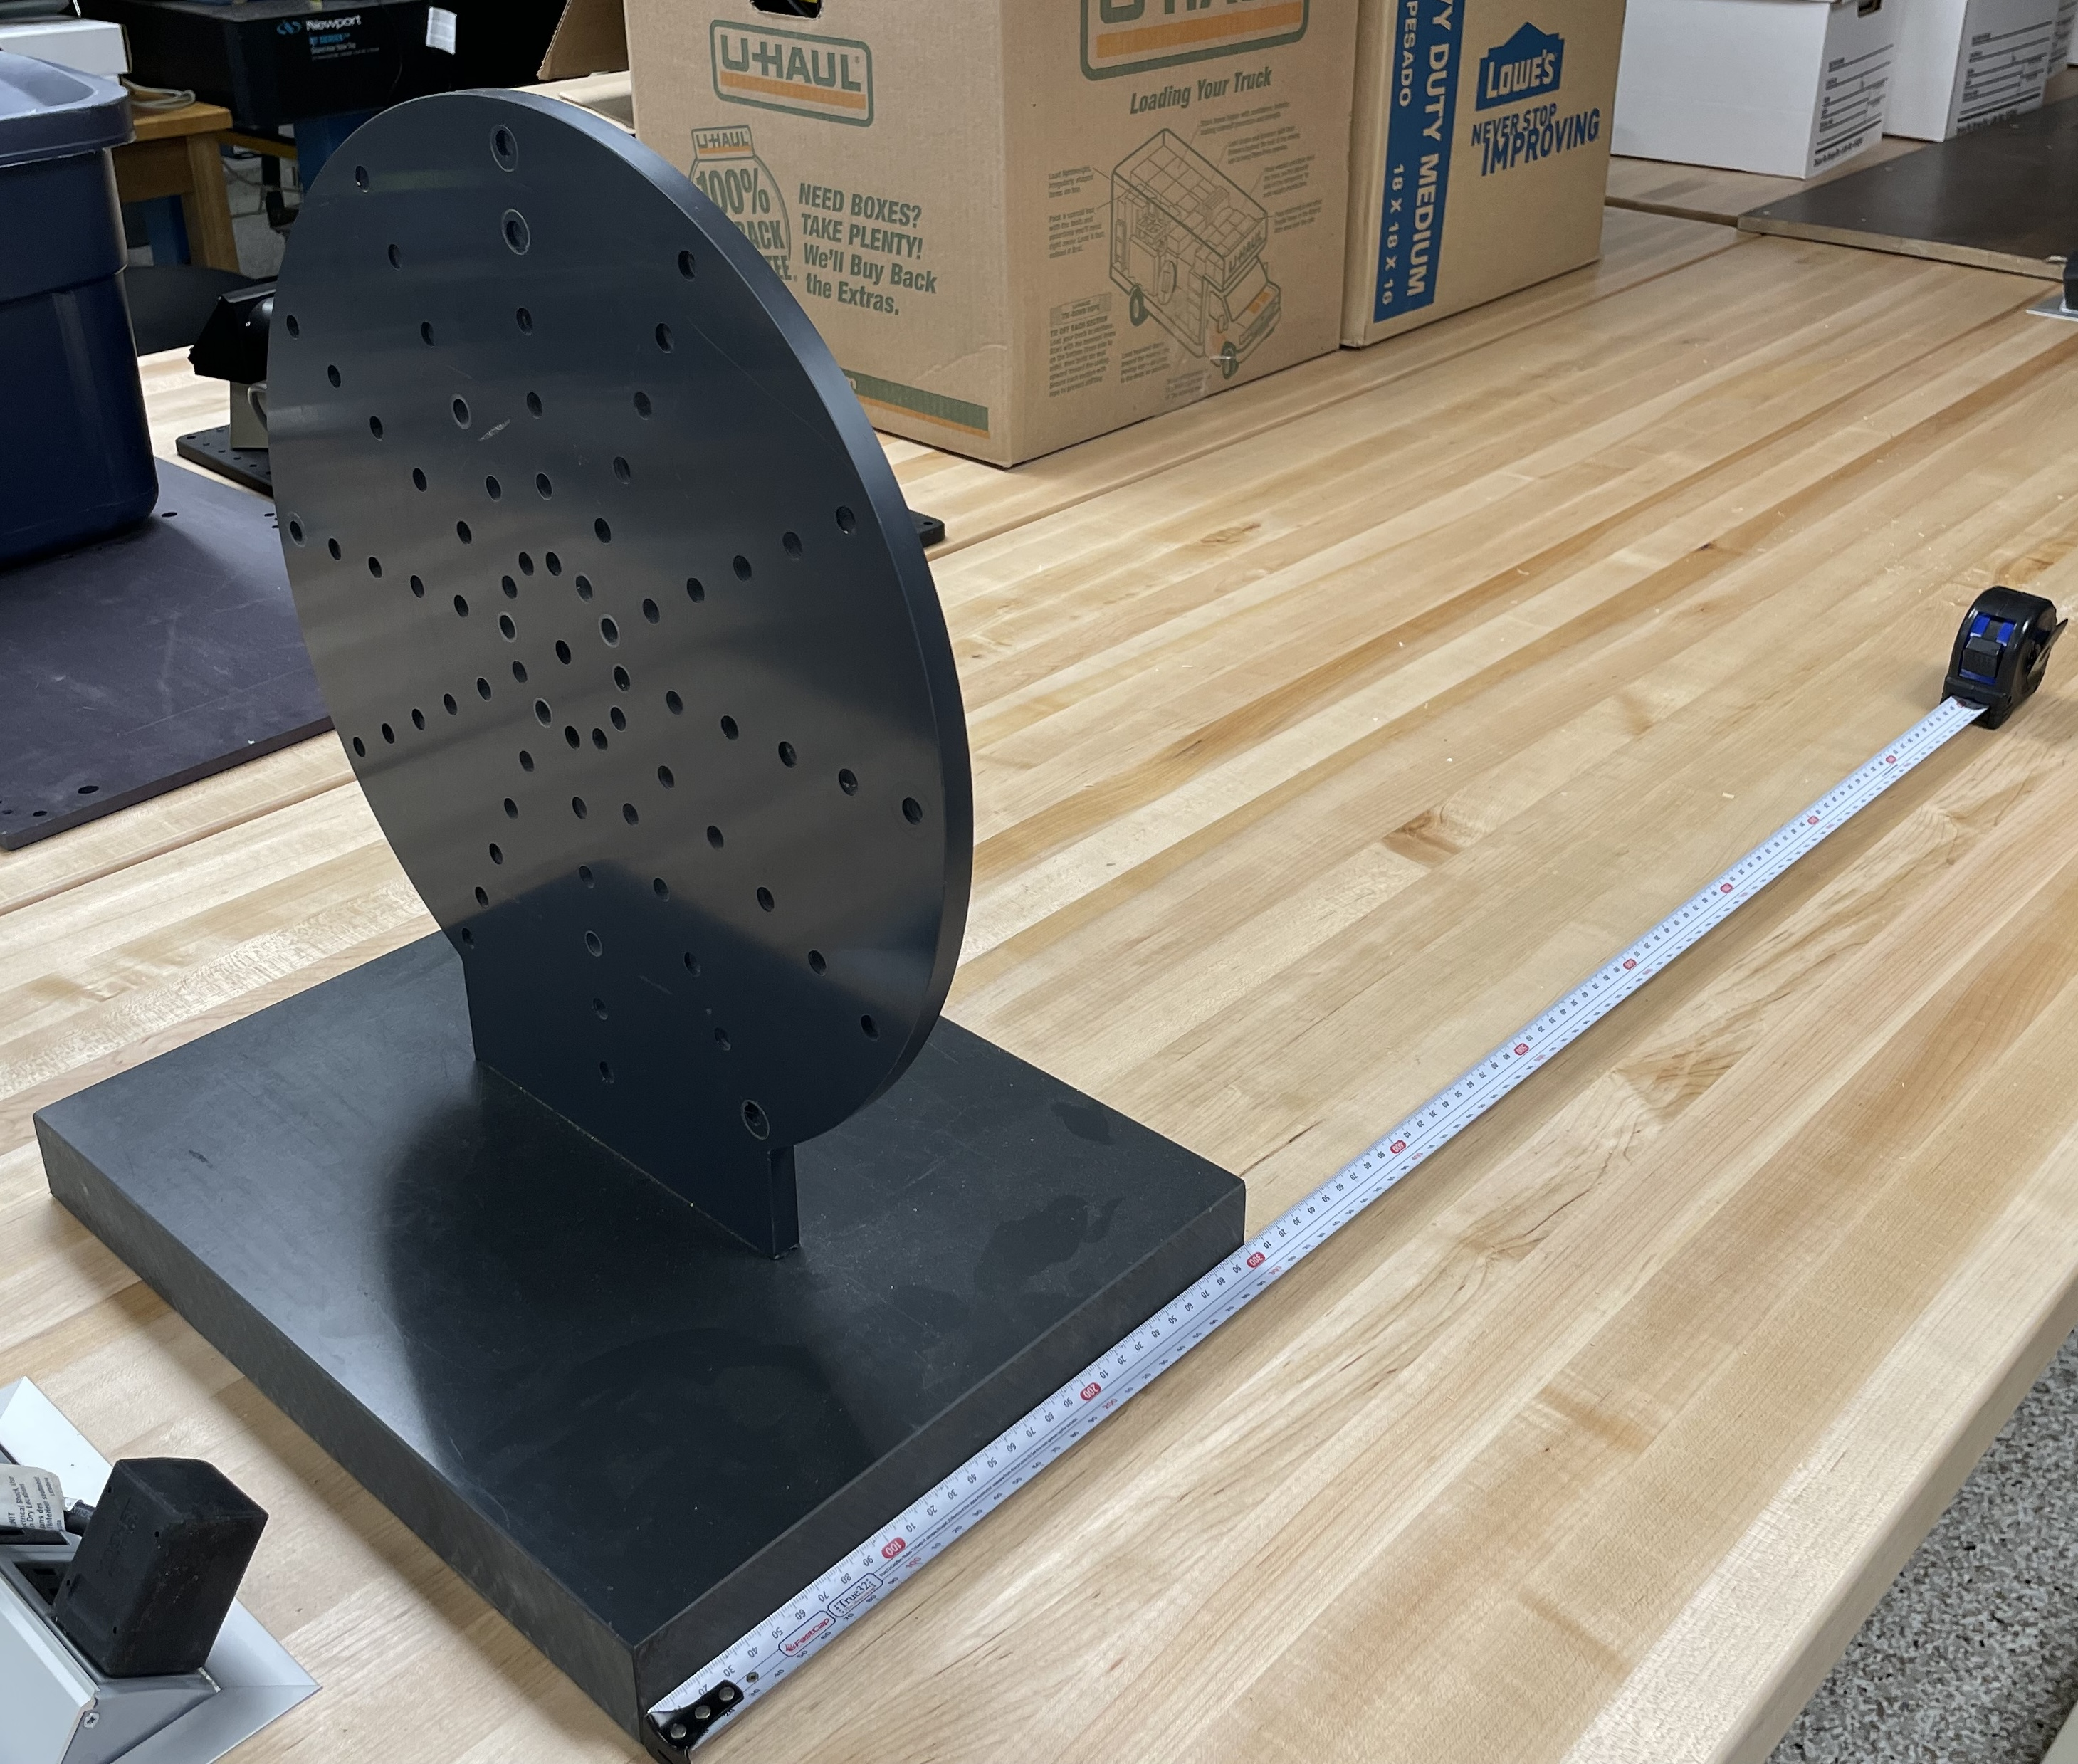
\includegraphics[width=\textwidth]{Assests/Picture3.jpg}
		\caption*{(a) PVC-based mapping platform.}
	\end{minipage}%
	\hfill
	\begin{minipage}[t]{0.48\textwidth}
		\centering
		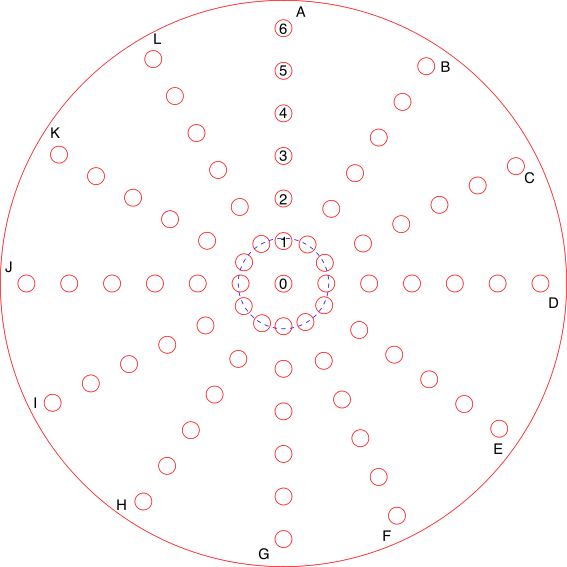
\includegraphics[width=0.85\textwidth]{Assests/MagFieldMap.png}
		\caption*{(b) Example field map output from MRI fringe region.}
	\end{minipage}
	\caption{PVC-based magnetic field mapping platform used for spatial $B_0$ and $\nabla B_0$ measurement. As shown in Ferreira 2017 \cite{haddixProposal,ferreira2017}.}
	\label{fig:fieldmapping}
\end{figure}


%LABVIEW program and Alpha Labs Protocols
Once the field‑mapping phantom and Gaussmeter probe are co‑aligned, data capture was streamlined to be sufficiently flexible and precise for our proximity measurements near an \gls{mri}. The manufacturer’s default software, AlphaApp, provides basic data‑logging, tethered or standalone recording, live screen streaming, and plotting of measurements from USB‑enabled AlphaLab meters\cite{AlphaApp}. However, AlphaApp **does not expose control over sampling frequency or allow real‑time adjustment of acquisition parameters**, limiting fine‑grained temporal resolution when the probe is moved into steep field gradients. In contrast, using \gls{lvi} interface allows for configurable sampling intervals, buffer control, and precise timing protocols, enabling us to push the device for much higher accuracy as the probe approaches and crosses isocontour regions within the \gls{mri} fringe. We developed that VI by leveraging the AlphaLab Data Acquisition Communication Protocol to command the device directly via USB, providing deterministic control over timing and sample rate \cite{AlphaAppProtocol}.

The data acquisition procedure for magnetic flux mapping is organized in this \gls{lvi}, whose basic logic is summarized in Figure~\ref{fig:gaussmeter-flowchart}. Upon startup, the \gls{lvi} initializes serial communication with the Gaussmeter, loads user-defined parameters (such as file name, mode of acquisition, delay time, and probe coordinates), and clears buffers in preparation for logging. The user may select either a continuous or an individual sampling mode. In continuous mode, the VI iterates through a defined number of data points with a fixed delay between samples; in individual mode, each data capture is triggered manually, allowing for precise positioning or timing. For both modes, each cycle involves reading the spatial coordinates, sending a measurement command, recording the returned magnetic flux value, and updating a graphical display as well as the output file.

While the flowchart reflects the core logic, it does not fully convey the customization added to the \gls{lvi} interface. For example, the front panel includes input fields for patient table (couch) parameters such as couch speed and displacement points. As mentioned above, our phantom is discretized with radial and angular indices: angular positions span 12 sectors clockwise from the 12 o’clock position (0 to 11 or A to L), and radial depths range from the center (0) to the outer edge (6). The probe’s spatial location is represented in polar coordinates, and the system plots magnetic flux as a function of position rather than time, allowing for intuitive visualization of the MRI fringe field across the phantom surface.

\begin{figure}[H]
	\centering
	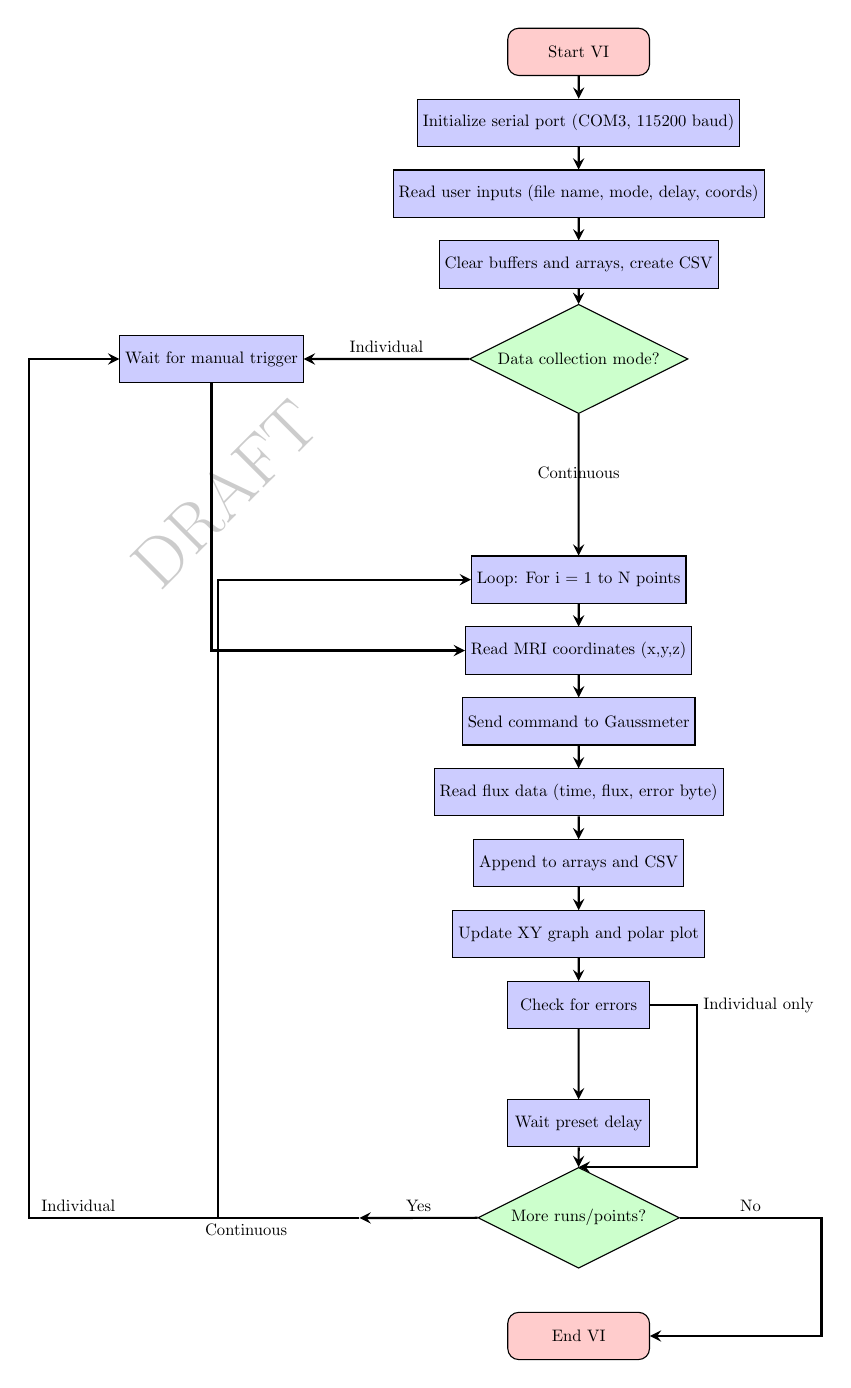
\begin{tikzpicture}[node distance=1.5cm, every node/.style={transform shape}, scale=0.6]
	
	% Start
	\node (start) [startstop] {Start VI};
	
	% Initialization
	\node (initserial) [process, below of=start] {Initialize serial port (COM3, 115200 baud)};
	\node (readinput) [process, below of=initserial] {Read user inputs (file name, mode, delay, coords)};
	\node (clearbuf) [process, below of=readinput] {Clear buffers and arrays, create CSV};
	
	% Mode decision
	\node (mode) [decision, below of=clearbuf, yshift=-0.5cm] {Data collection mode?};
	
	% Individual branch: manual trigger wait before data steps
	\node (manualTrigger) [process, left=3.5cm of mode] {Wait for manual trigger};
	
	%Continuous loop
	\node (loopCount) [process, below =3cm of mode] {Loop: For i = 1 to N points};
	
	% Data acquisition steps (common)
	\node (readcoords) [process, below of=loopCount] {Read MRI coordinates (x,y,z)};
	\node (sendcmd) [process, below of=readcoords] {Send command to Gaussmeter};
	\node (readflux) [process, below of=sendcmd] {Read flux data (time, flux, error byte)};
	\node (store) [process, below of=readflux] {Append to arrays and CSV};
	\node (updateplots) [process, below of=store] {Update XY graph and polar plot};
	\node (checkerrors) [process, below of=updateplots] {Check for errors};
	
	% Continuous mode: wait delay after error check
	\node (delayWait) [process, below of=checkerrors, yshift=-1cm] {Wait preset delay};

	
	% Loop decision
	\node (moreRuns) [decision, below of=delayWait, yshift=-0.5cm] {More runs/points?};
	
	% End
	\node (end) [startstop, below of=moreRuns, yshift=-1cm] {End VI};
	
	% Arrows: initialization flow
	\draw [arrow] (start) -- (initserial);
	\draw [arrow] (initserial) -- (readinput);
	\draw [arrow] (readinput) -- (clearbuf);
	\draw [arrow] (clearbuf) -- (mode);
	
	% Mode branches
	\draw [arrow] (mode) -- node[above] {Individual} (manualTrigger);
	\draw [arrow] (mode) -- node[above] {Continuous} (loopCount);
	
	% Individual flow to data steps
	\draw [arrow] (manualTrigger) |- (readcoords.west);
	
	% Data acquisition common flow
	\draw [arrow] (loopCount) -- (readcoords);
	\draw [arrow] (readcoords) -- (sendcmd);
	\draw [arrow] (sendcmd) -- (readflux);
	\draw [arrow] (readflux) -- (store);
	\draw [arrow] (store) -- (updateplots);
	\draw [arrow] (updateplots) -- (checkerrors);
	
	% Continuous flow: after errors wait delay, then loop decision
	\draw [arrow] (checkerrors) -- (delayWait);
	\draw [arrow] (delayWait) -- (moreRuns);
	
	% Individual flow: after errors go directly to loop decision (skip delay)
	\draw [arrow] (checkerrors.east) -- ++(1,0) node[pos=0.3, right, xshift=20pt] {Individual only} |- (moreRuns.north);

	% Loop decision arrows:
	% If yes, loop back to the start of the mode branch
	% Intermediate branch point for Yes
	\node (yesBranch) [coordinate, left=2.5cm of moreRuns.west] {};
	
	% Arrow from moreRuns to yesBranch labeled "Yes"
	\draw [arrow] (moreRuns.west) -- node[midway, above] {Yes} (yesBranch);
	
	% Branch to Individual
	\draw [arrow] (yesBranch) -- node[pos=0.85,above] {Individual} ++(-7,0) |- (manualTrigger.west);
	
	% Branch to Continuous
	\draw [arrow] (yesBranch) -- node[pos=0.8,below] {Continuous} ++(-3,0) |- (loopCount.west);


	
	% If no, end program
	\draw [arrow] (moreRuns.east) -- node[midway, above] {No} ++(3,0) |- (end.east);
	
\end{tikzpicture}
	\caption{Flowchart of the Gaussmeter VI data acquisition algorithm.}
	\label{fig:gaussmeter-flowchart}
\end{figure}

In clinical use, the entire fixture is intended to be shifted axially along the Z-direction of a horizontal bore MRI scanner using controlled couch increments (e.g., 10 cm). This translation allows for volumetric sampling of $B_0$ over several planes. The spatial magnetic field gradient$\nabla B_0$ can then be estimated numerically using finite difference calculations between adjacent measurement points. This method has previously been applied to MRI mapping in the work by Ferreira \cite{ferreira2017}.





\subsection{Translational Force Measurement via Angular Deflection}

\subsubsection{Laboratory Simulation with Solenoid Coil}

To assess MRI-induced translational forces in a laboratory environment, Creighton University developed a pendulum-style apparatus following the geometry and physics outlined in ASTM F2052-15\cite{astmF2052}. The vertical post includes a screw clamp mechanism that enables height adjustment; however, a default suspension height of 1 meter was used for consistency across trials.

The experimental frame was constructed entirely from \gls{pvc} components (Figure \ref{fig:schematic}a), including a vertical post of 1.5 meters and a rigid base for stabilization. The sample—a \textbf{solid ferromagnetic cylinder} (length = 6 mm, diameter = 3 mm, mass = 0.3648 g, density = 8.6 g/cm$^3$)—was suspended by a \textbf{955 mm-long sewing thread}, tied via a simple knot at its center. For clinical applications, a \textbf{0.25 mm nylon monofilament} is recommended for improved reproducibility and safety. A Monofilament Nylon thread has low stretch,  complies with MR-safe properties (Non-metallic, Non-conductive, Non-magnetic), and reduces variability introduced by torsional drift or thread elasticity  \cite{stoianovici2024, astmF2052}. The bottom of the sample was free to swing, forming a pendulum under gravity. A horizontal ruler, fixed along the Z-axis, served as the visual reference to quantify lateral displacements as shown in Figure \ref{fig:schematic}b and detailed in Figure~\ref{fig:leadcloseup}. 


\begin{figure}[H]
	\centering
	\begin{minipage}[b]{0.48\textwidth}
		\centering
		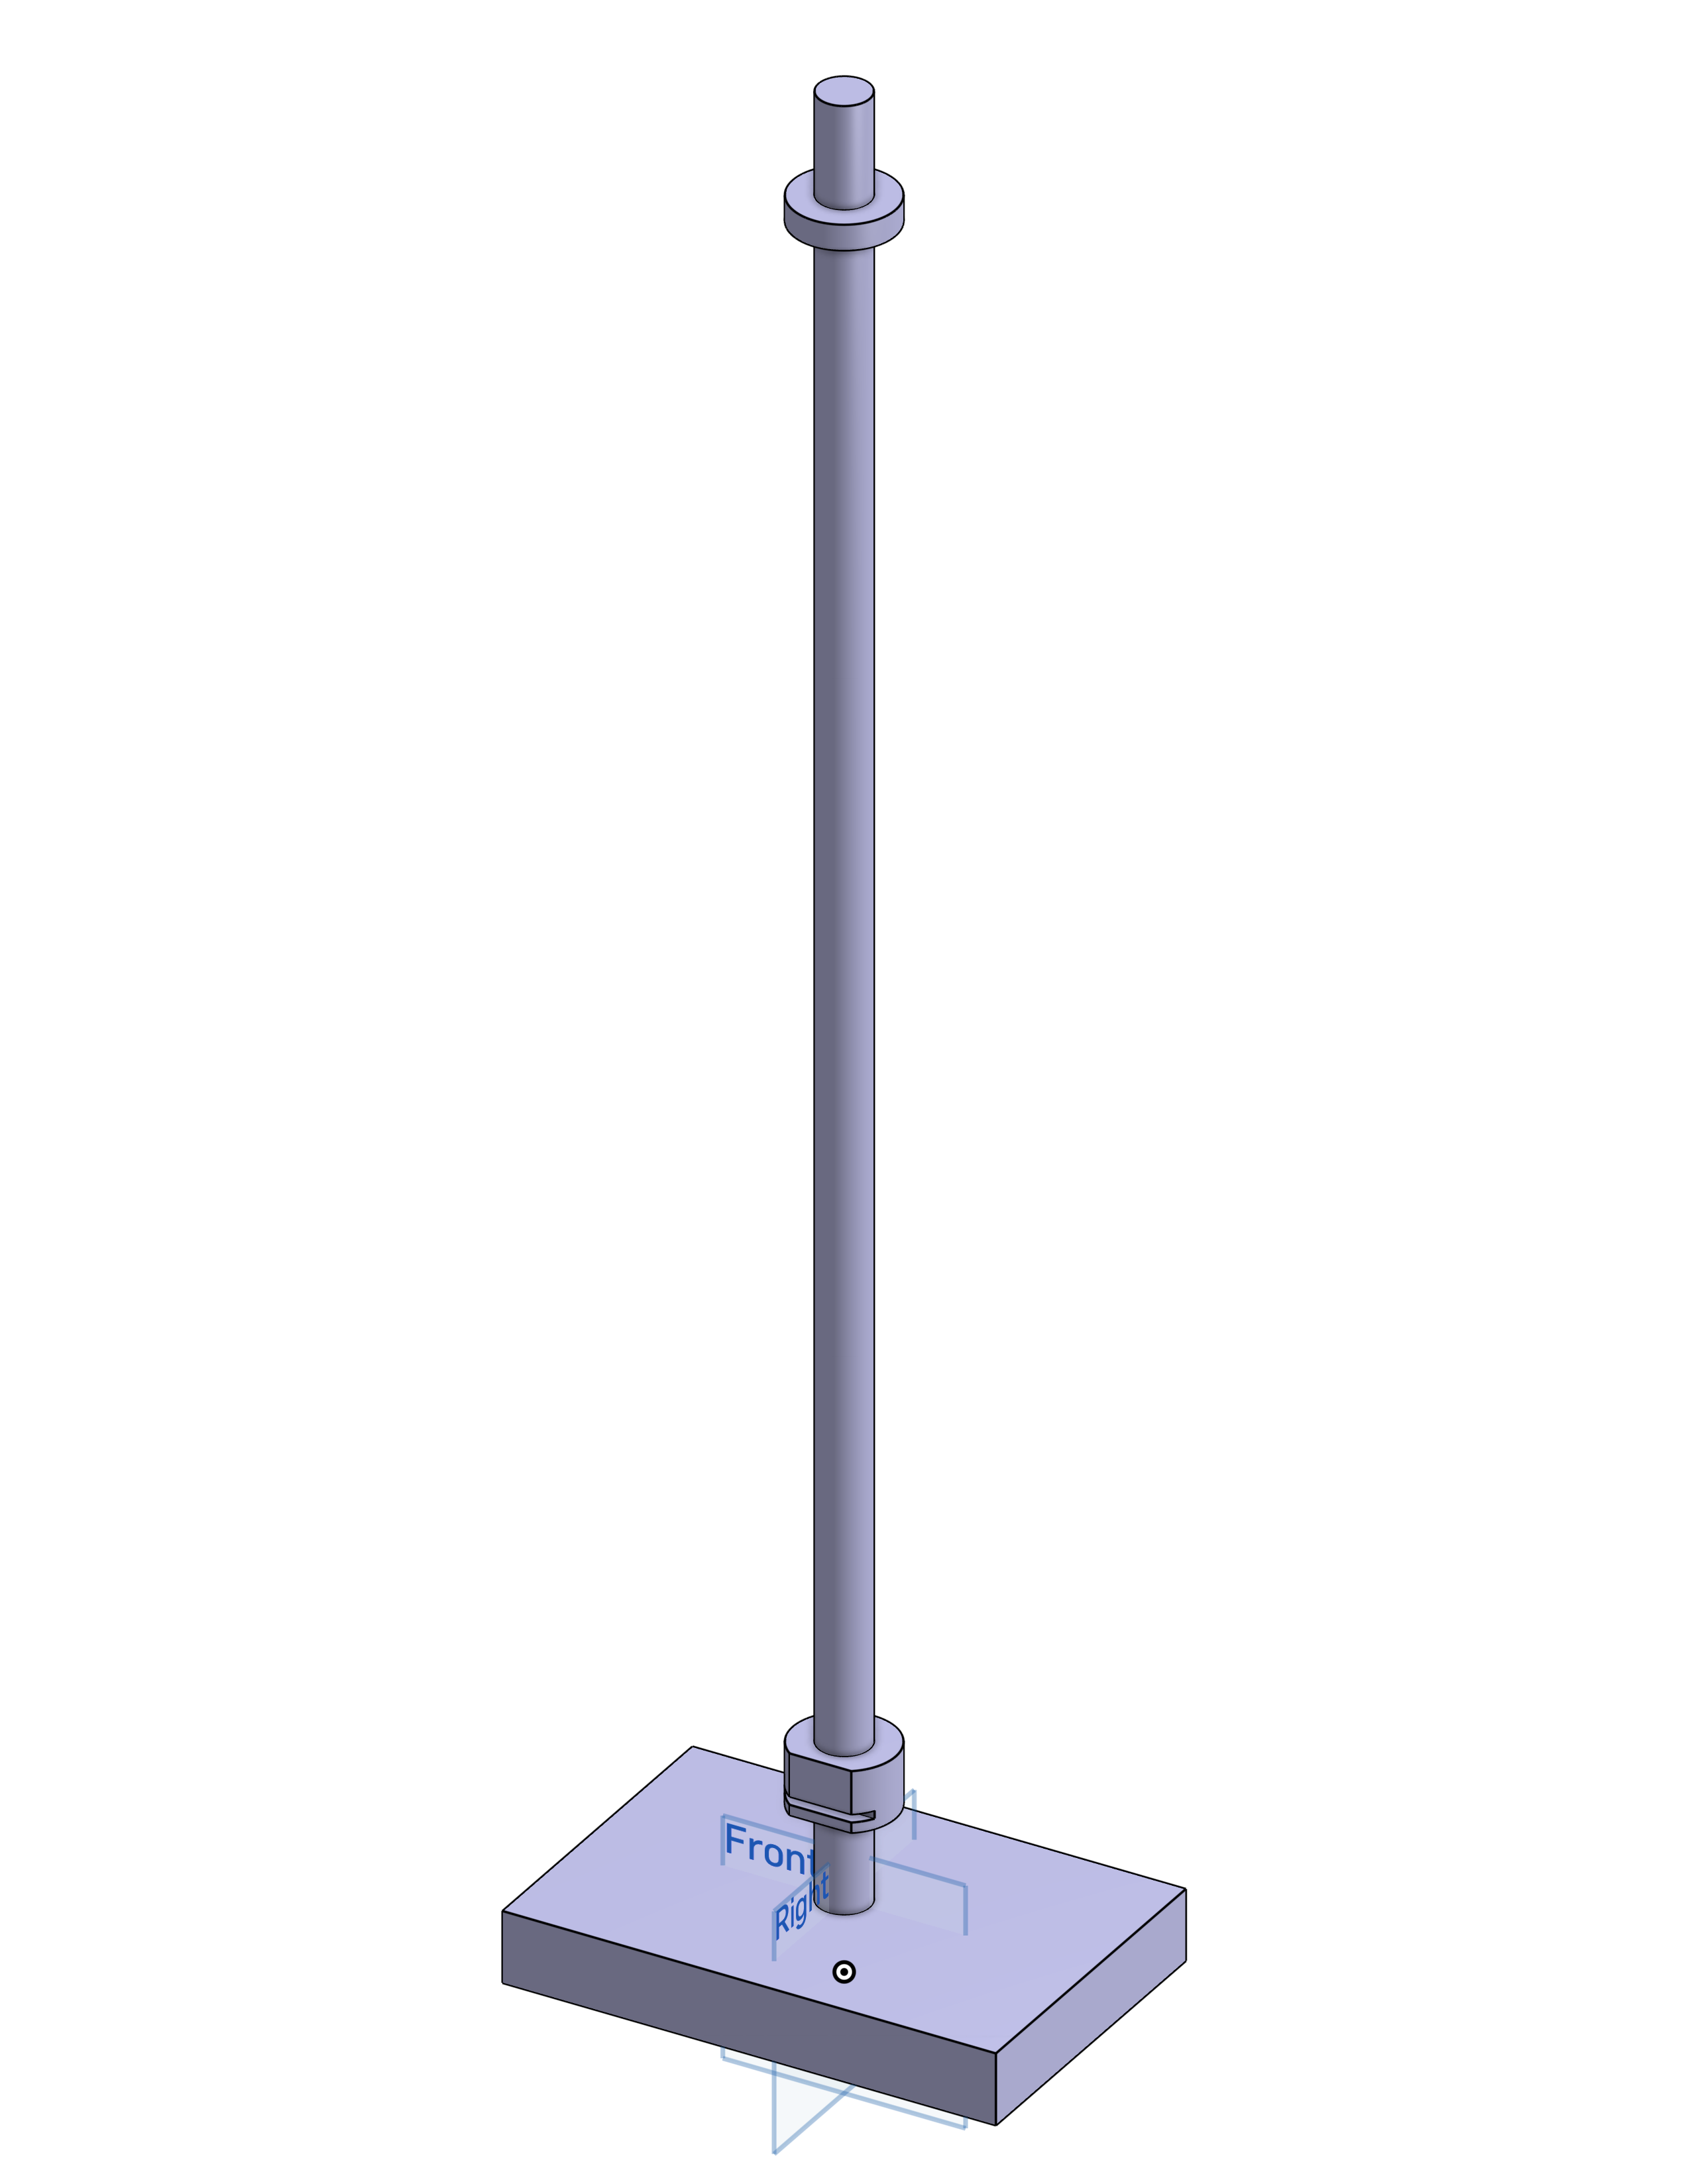
\includegraphics[width=\textwidth]{Assests/Part1.png}
		\subcaption{CAD render of the pendulum apparatus created using CATIA.}
	\end{minipage}
	\hfill
	\begin{minipage}[b]{0.48\textwidth}
		\centering
		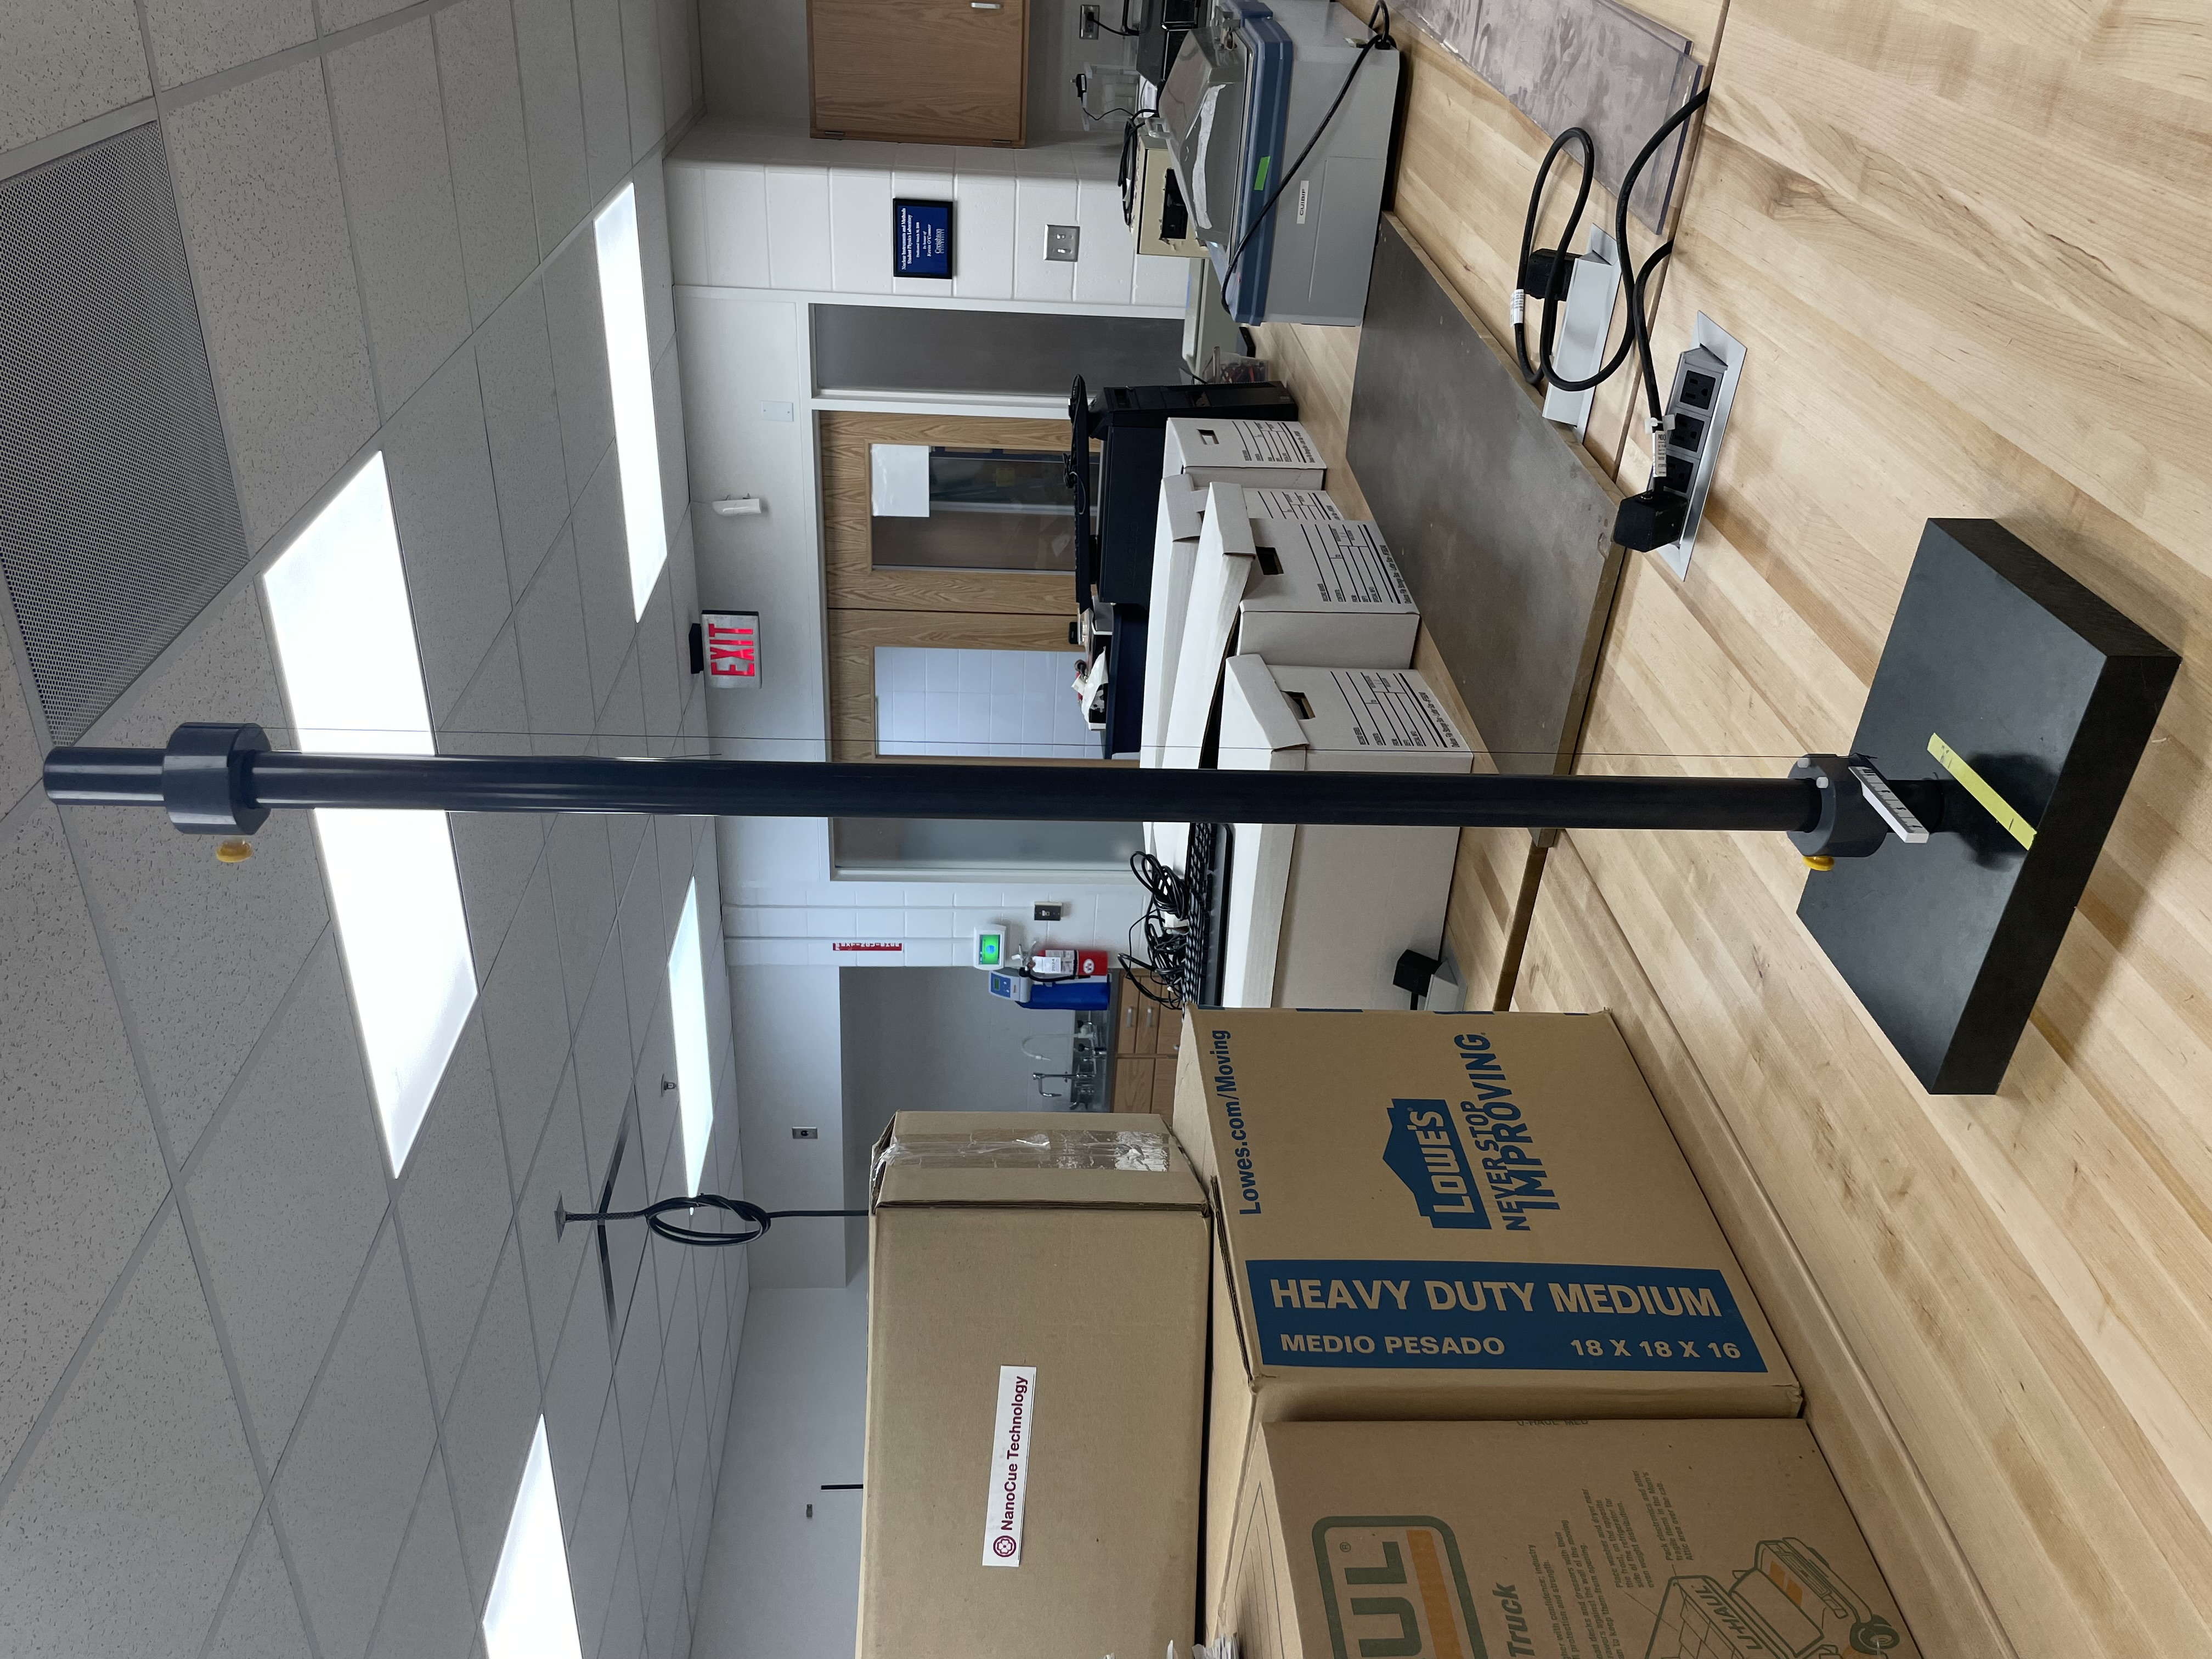
\includegraphics[width=1.3\textwidth, angle=-90]{Assests/Picture1.jpg}
		\subcaption{Real-life implementation of the apparatus in the laboratory setting.}
	\end{minipage}
	\caption{Experimental pendulum-based apparatus constructed from PVC for MRI translational force measurements.}
	\label{fig:schematic}
\end{figure}

\subsubsection*{Lead Holder Frame Design}

To accommodate epicardial lead positioning while maintaining MRI compatibility, we propose the use of a lightweight, non-magnetic bee comb mesh also fabricated from \gls{pla}. The suggested mesh dimensions are 16 mm length by 14 mm wide, with a thickness of 1 mm, for a total volume of less than $100 mm^3$ equivalent to around a tenth of 1 gram given the 1.24 grams per cubic centimeter ($g/cm^3$) \gls{pla} density. 

As shown in figure \ref{fig:leadHolder} and \ref{fig:leadcloseup}.

The mesh needs to be suspended such that the lead axis was aligned approximately parallel to the magnetic field gradient (Z-axis). The mesh's lightweight design aimed to minimize its contribution to the total magnetic force, however its mass was not explicitly subtracted from the translational force calculations.

\begin{figure}[H]
	\centering
	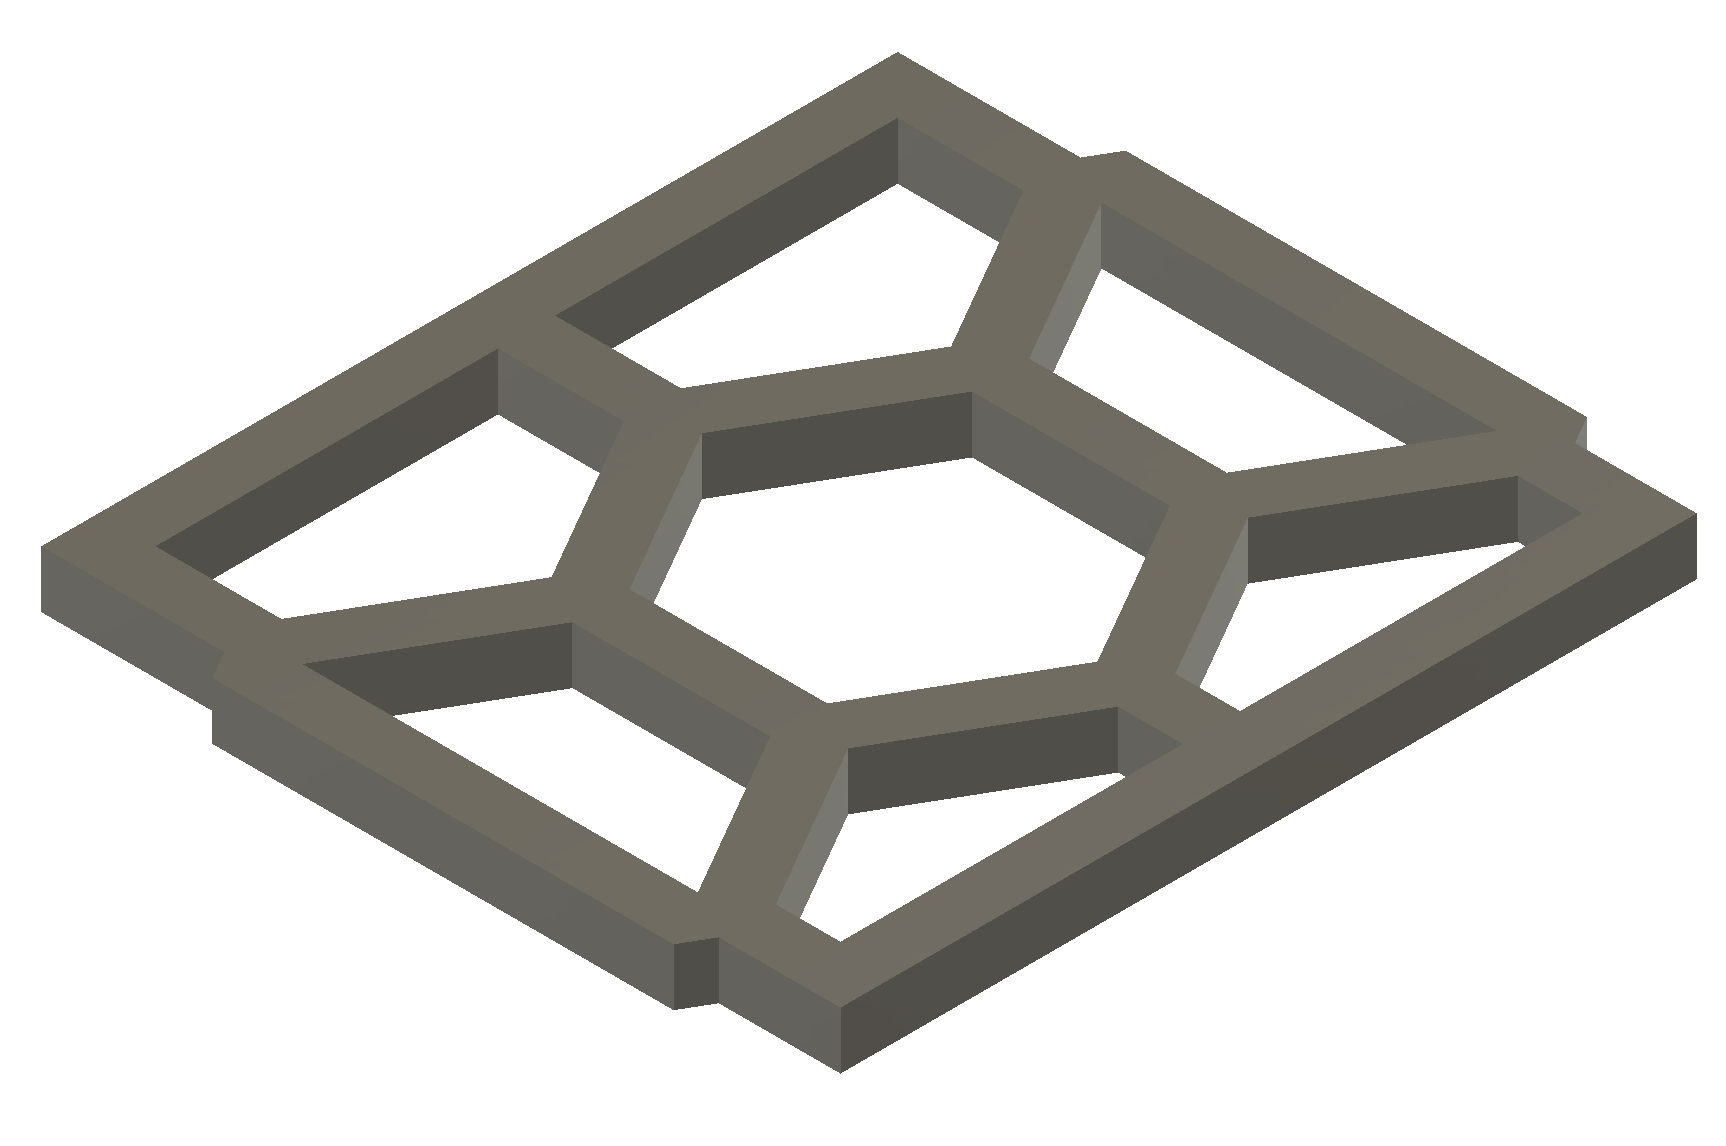
\includegraphics[width=0.5\textwidth]{Assests/frameHolder.png}
	\caption[3D render of the design on lead holder]{The design on lead holder comprises a rectangular lightweight bee comb mesh to wrap the epicardial lead around and hold it in a pendulum with a nylon string}	
	\label{fig:leadHolder}
\end{figure}

A summary schematic of the apparatus and frame are included in Figures \ref{fig:schematic} and \ref{fig:leadHolder}, with additional engineering drawings available in %\textbf{\AppendixAone} and \textbf{\AppendixAtwo}.



\begin{figure}[H]
	\centering
	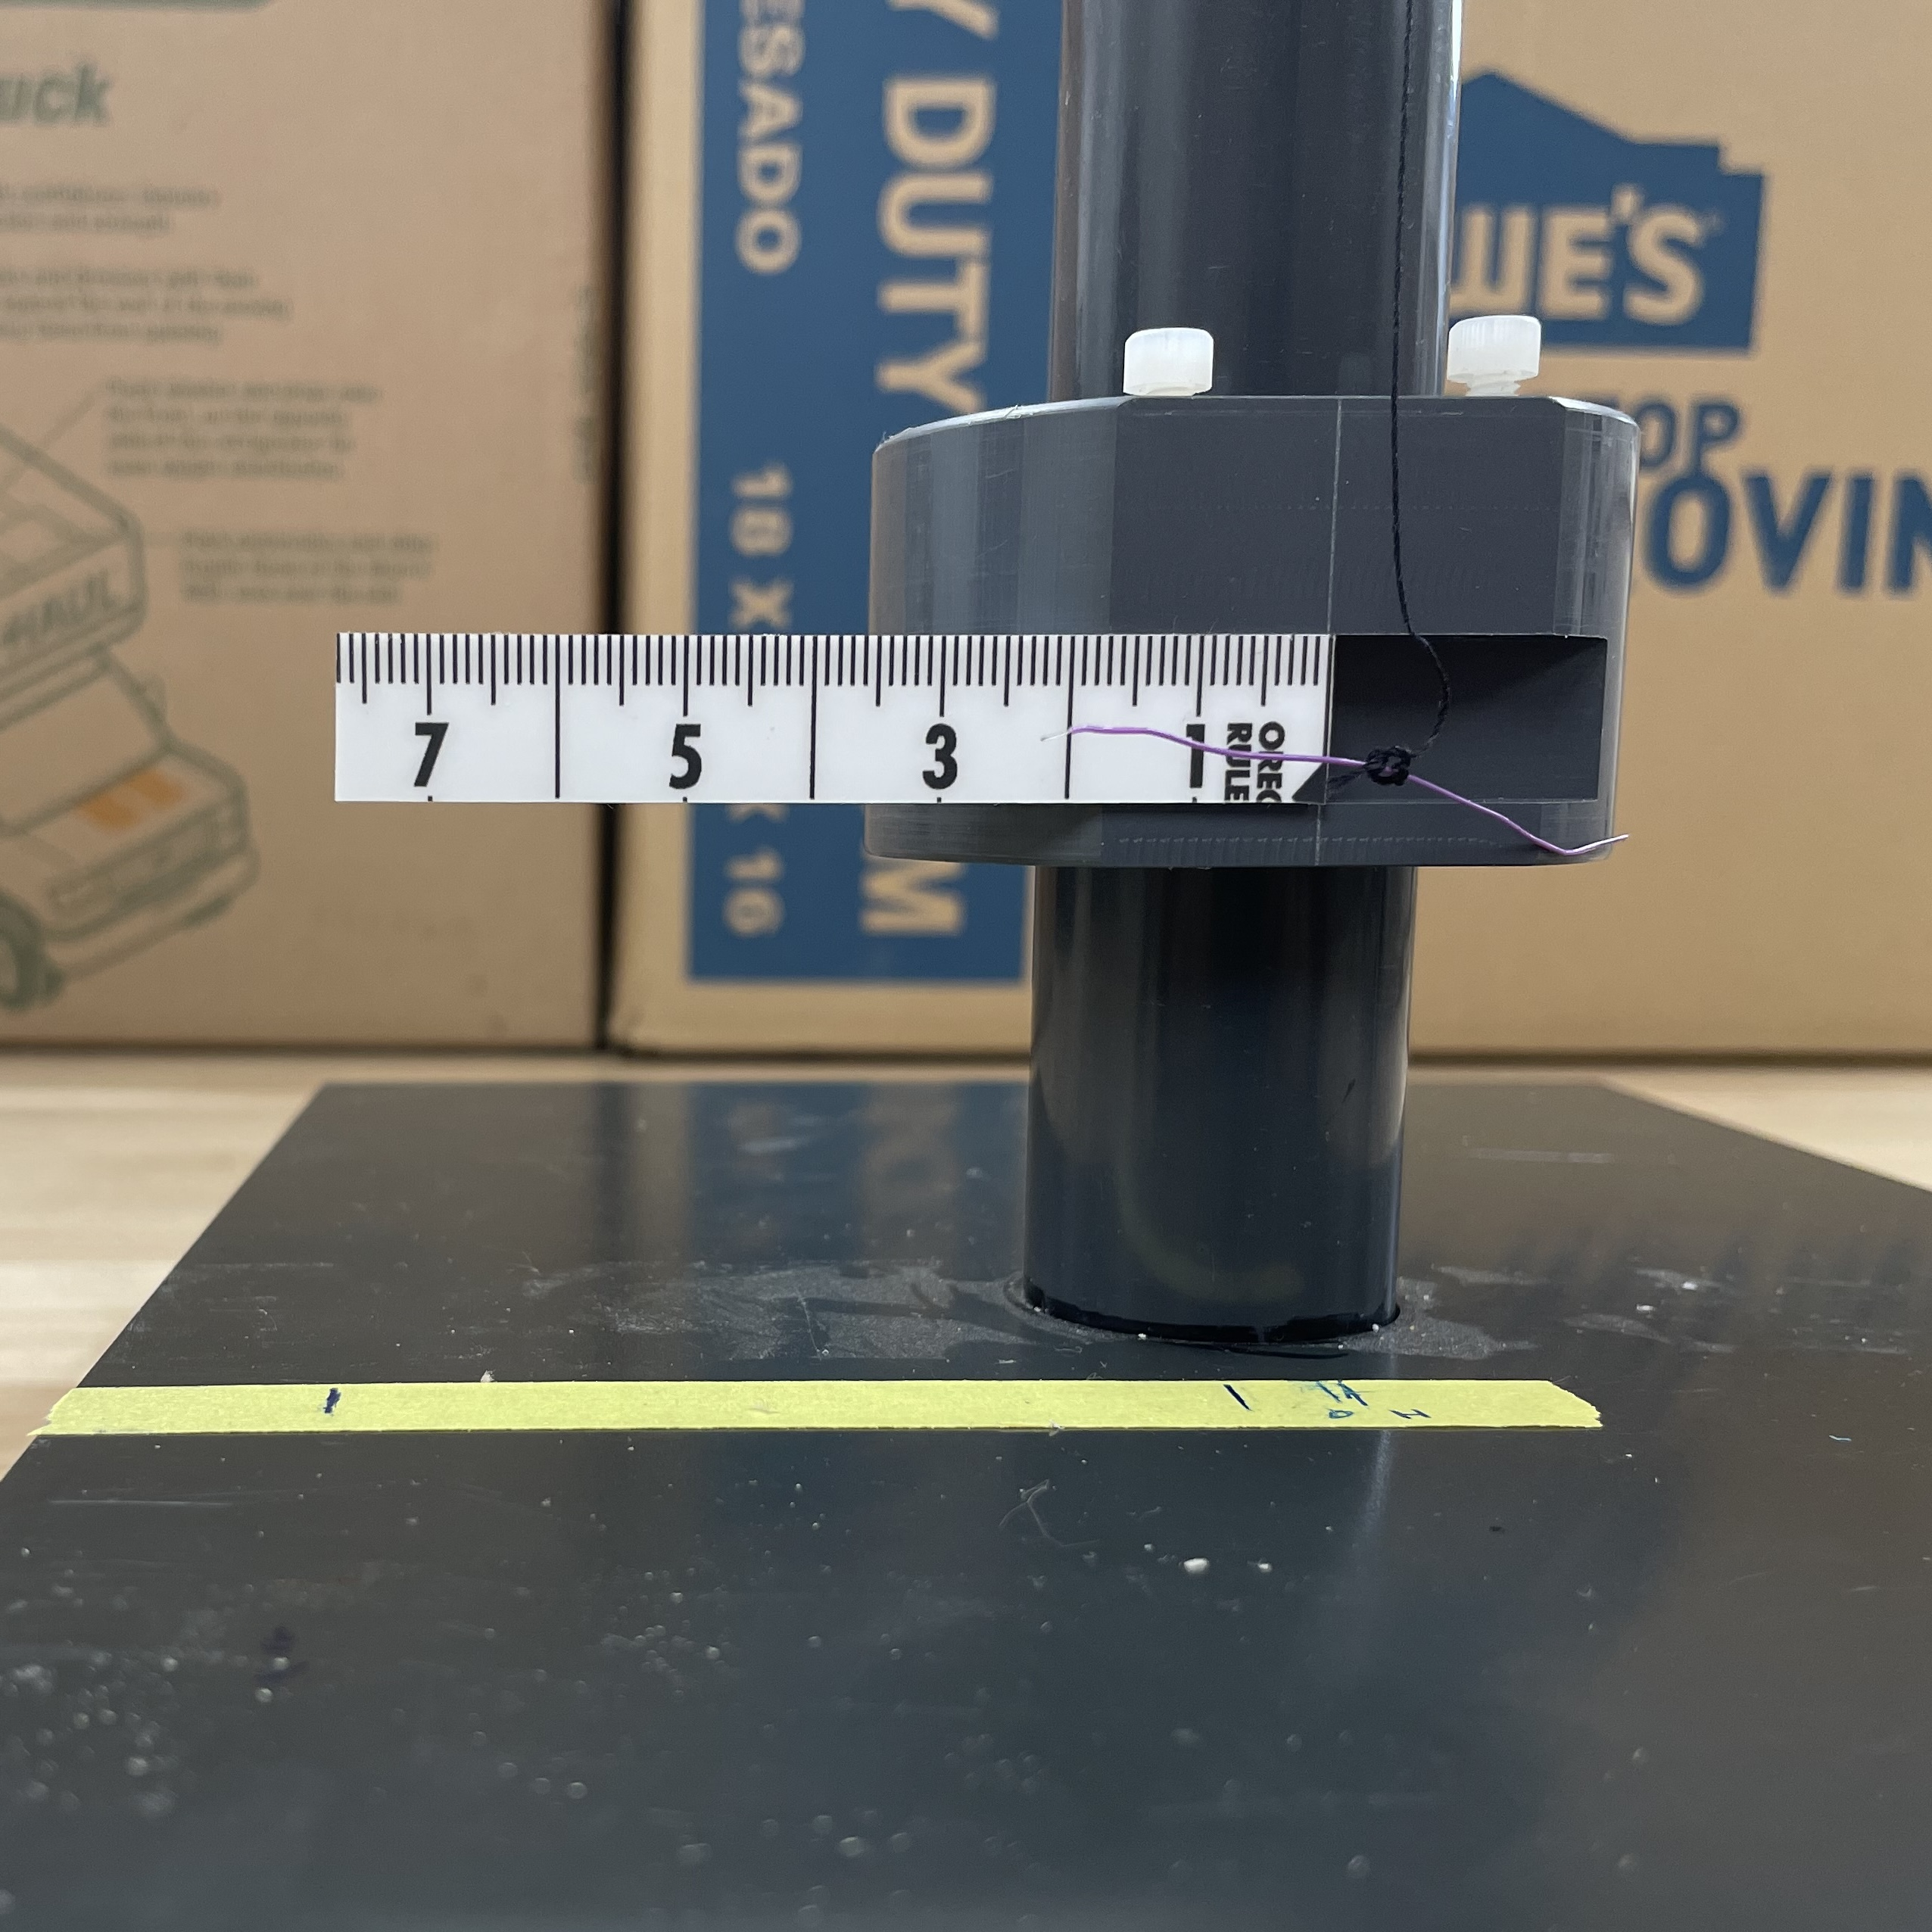
\includegraphics[width=0.6\textwidth]{Assests/Picture2.jpg}
	\caption{Close-up of the epicardial lead fragment suspended by monofilament thread over the ruler. Image illustrates the displacement measurement system and the sample scale.}
	\label{fig:leadcloseup}
\end{figure}

\subsubsection*{In Lab Measurement Protocol}

Magnetic field measurements were performed using the \textbf{AlphaLab Inc. Gaussmeter} described before. To characterize local field gradients, measurements were taken at three positions: at the pendulum's equilibrium position, 0.5 mm below, and 0.5 mm above, yielding values of $B_{-0.5}$, $B_0$, and $B_{+0.5}$, respectively. Each position was sampled \textbf{nine times per current level}, and gradients were computed using python pandas library and the central finite difference method:

\begin{equation}
	\frac{dB}{dz} \approx \frac{B_{+0.5} - B_{-0.5}}{1\ \text{mm}}
\end{equation}

Once the pendulum reached equilibrium under each magnetic condition, the horizontal displacement on $z$ was recorded visually using the ruler as a reference. With known suspension length $L$, the \textbf{deflection angle $\alpha$} was calculated as:

\begin{equation}
	\alpha = \tan^{-1}\left(\frac{x}{L}\right)
\end{equation}

Following ASTM F2052-15, the translational force exerted on a device due to a static magnetic field spatial gradient can be evaluated through angular deflection. In this setup, the test object is suspended in equilibrium, and the balance of forces leads to:

\begin{equation}
	\tan \alpha = \frac{F_m}{mg}
\end{equation}

where $\alpha$ is the deflection angle from vertical, $F_m$ is the magnetically induced translational force, $m$ is the mass of the object, and $g$ is the gravitational acceleration. Rearranging gives:

\begin{equation}
	F_m = mg \tan \alpha
\end{equation}

This is also derived from Newtonian force balancing as in Appendix X2 of ASTM F2052-15 (Fig \ref{fig:astm_diagram}), and is valid even in cases when the magnetic force does not operate exactly at the center of mass. As a result, the approach is reliable for evaluating a variety of devices.

\begin{figure}[htbp]
	\centering
	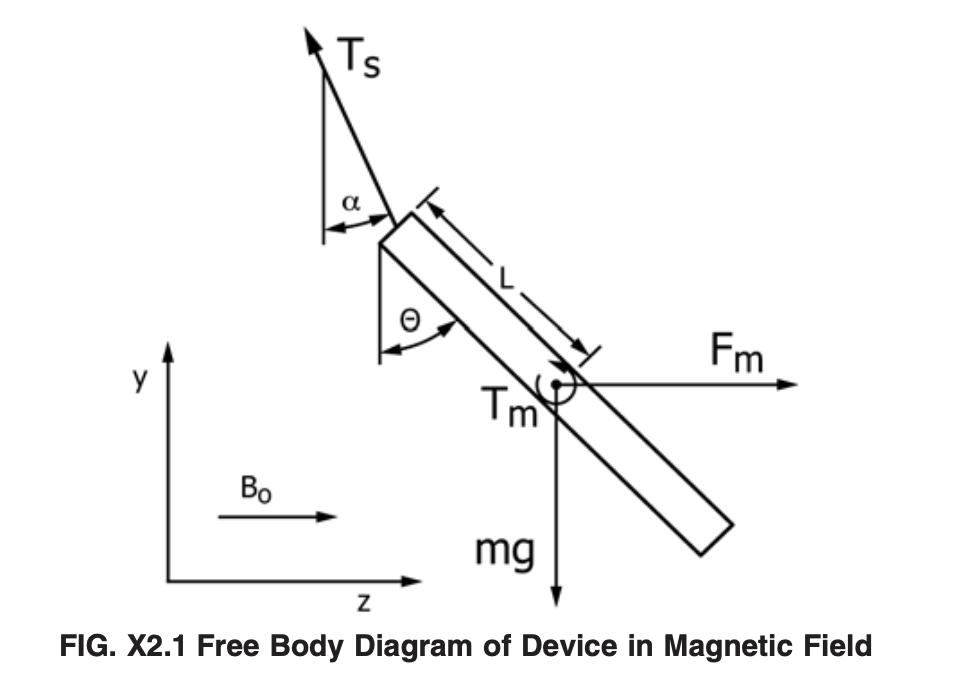
\includegraphics[width=0.6\textwidth]{Assests/astm_diagram.png}
	\caption{Free-body diagram of device in magnetic field (adapted from ASTM F2052-15, Appendix X2).}
	\label{fig:astm_diagram}
\end{figure}

For materials where magnetization is induced by a static field (e.g., paramagnetic or unsaturated ferromagnetic materials), the translational force can also be expressed in terms of volumetric magnetic susceptibility $\chi$, assuming linear response:

\begin{equation}
	F_m = \frac{\chi V}{\mu_0} B_0 \frac{dB_0}{dz}
	\quad \Rightarrow \quad
	\chi = \frac{\mu_0 F_m}{V B_0 \frac{dB_0}{dz}}
\end{equation}

Combining this with the earlier result:

\begin{equation}
	\chi = \frac{\mu_0 m g \tan \alpha}{V B_0 \frac{dB_0}{dz}}
\end{equation}

This provides a direct estimation of magnetic susceptibility from angular deflection measurements, provided the field and its gradient are known. 

The ratio is expressed as follows using a different, dimensionally reduced form from ASTM F2052-15's Appendix X3:

\begin{equation}
	\frac{\chi}{\rho \mu_0 g} = \frac{\tan \alpha}{B_0 \frac{dB_0}{dz}}
\end{equation}

This formulation explains why the measured deflection angle $\alpha$ (and thus $F_m$) depends not on $\chi$ or $B_0$ independently, but on their product. Practically, this insight justifies our lab methodology: although our solenoid generates only ~20 Gauss, we used a highly ferromagnetic sample (large $\chi$), allowing us to replicate clinically relevant force-to-weight ratios ($F_m / mg$).

In the clinical MRI environment, $B_0$ may reach 3 T, but the $\chi$ of implanted materials is often orders of magnitude smaller. This inverse balance preserves the translational force regime, and supports translating results from lab simulations to clinical conditions.

%\subsection*{Data Collection and Analysis}

All measurements were logged in \textbf{Microsoft Excel}, and photos/videos were captured via smartphone to document behavior. A minimum of \textbf{three trials} were performed for each current level; however, only the final (most consistent) dataset was retained for analysis. Data were exported to a Jupyter Notebook for clean up and processing with pandas. Then plotted to evaluate $\tan \alpha$ vs. field gradient force. Propagated uncertainties in $\alpha$ and $dB_0/dz$ were computed using standard error propagation formulas.

\subsubsection{In Clinic Measurement Protocol}




\subsection{Torque Measurement Apparatus (In Progress)}

A torque measurement system based on ASTM F2213 is under development. While a prototype was fabricated under the supervision of Dr. Nichols and prior students, detailed calibration, operational workflow, and data acquisition methods are still being finalized. The system is expected to allow both qualitative torque threshold assessments and quantitative torque calculation by assessing rotational displacement under a known static field. This device is shown in figure \ref{fig:torqueDevice}.


\begin{figure}[H]
	\centering
	\begin{minipage}[b]{0.48\textwidth}
		\centering
		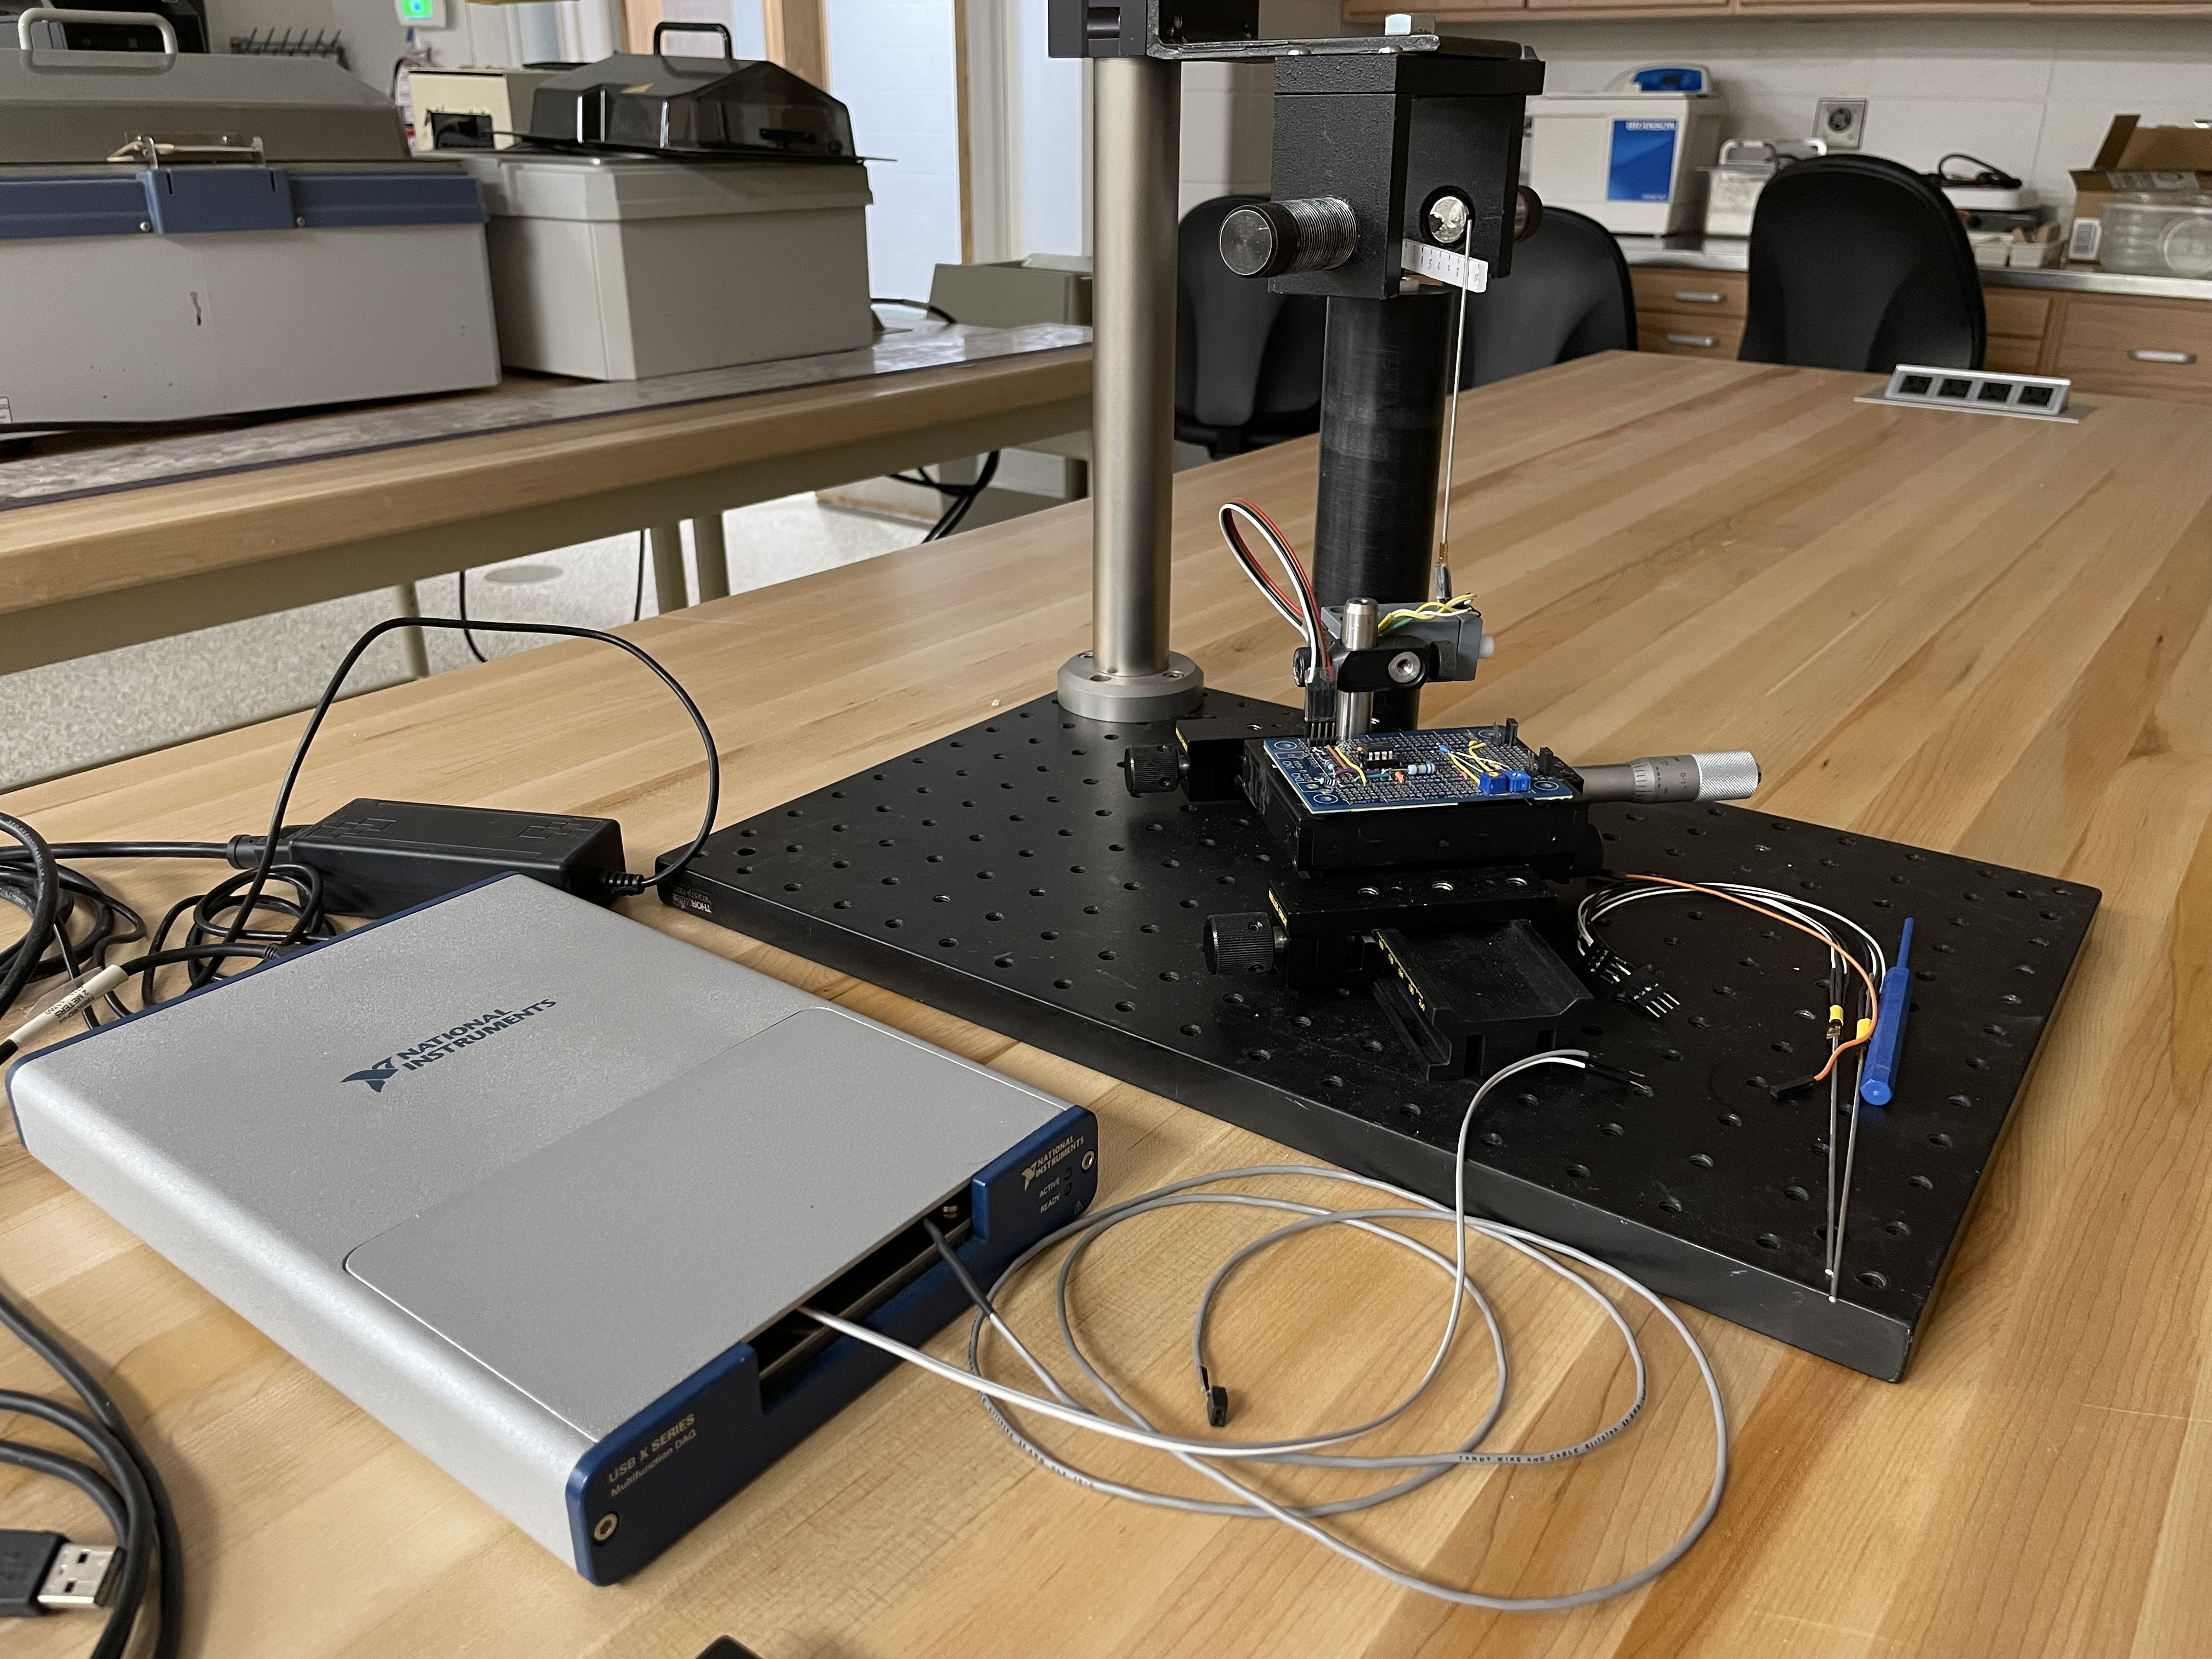
\includegraphics[width=\textwidth]{Assests/torquesDev.jpg}
		\subcaption{Current torque measurement device}
		\vspace{0.95cm}
	\end{minipage}
	\hfill
	\begin{minipage}[b]{0.48\textwidth}
		\centering
		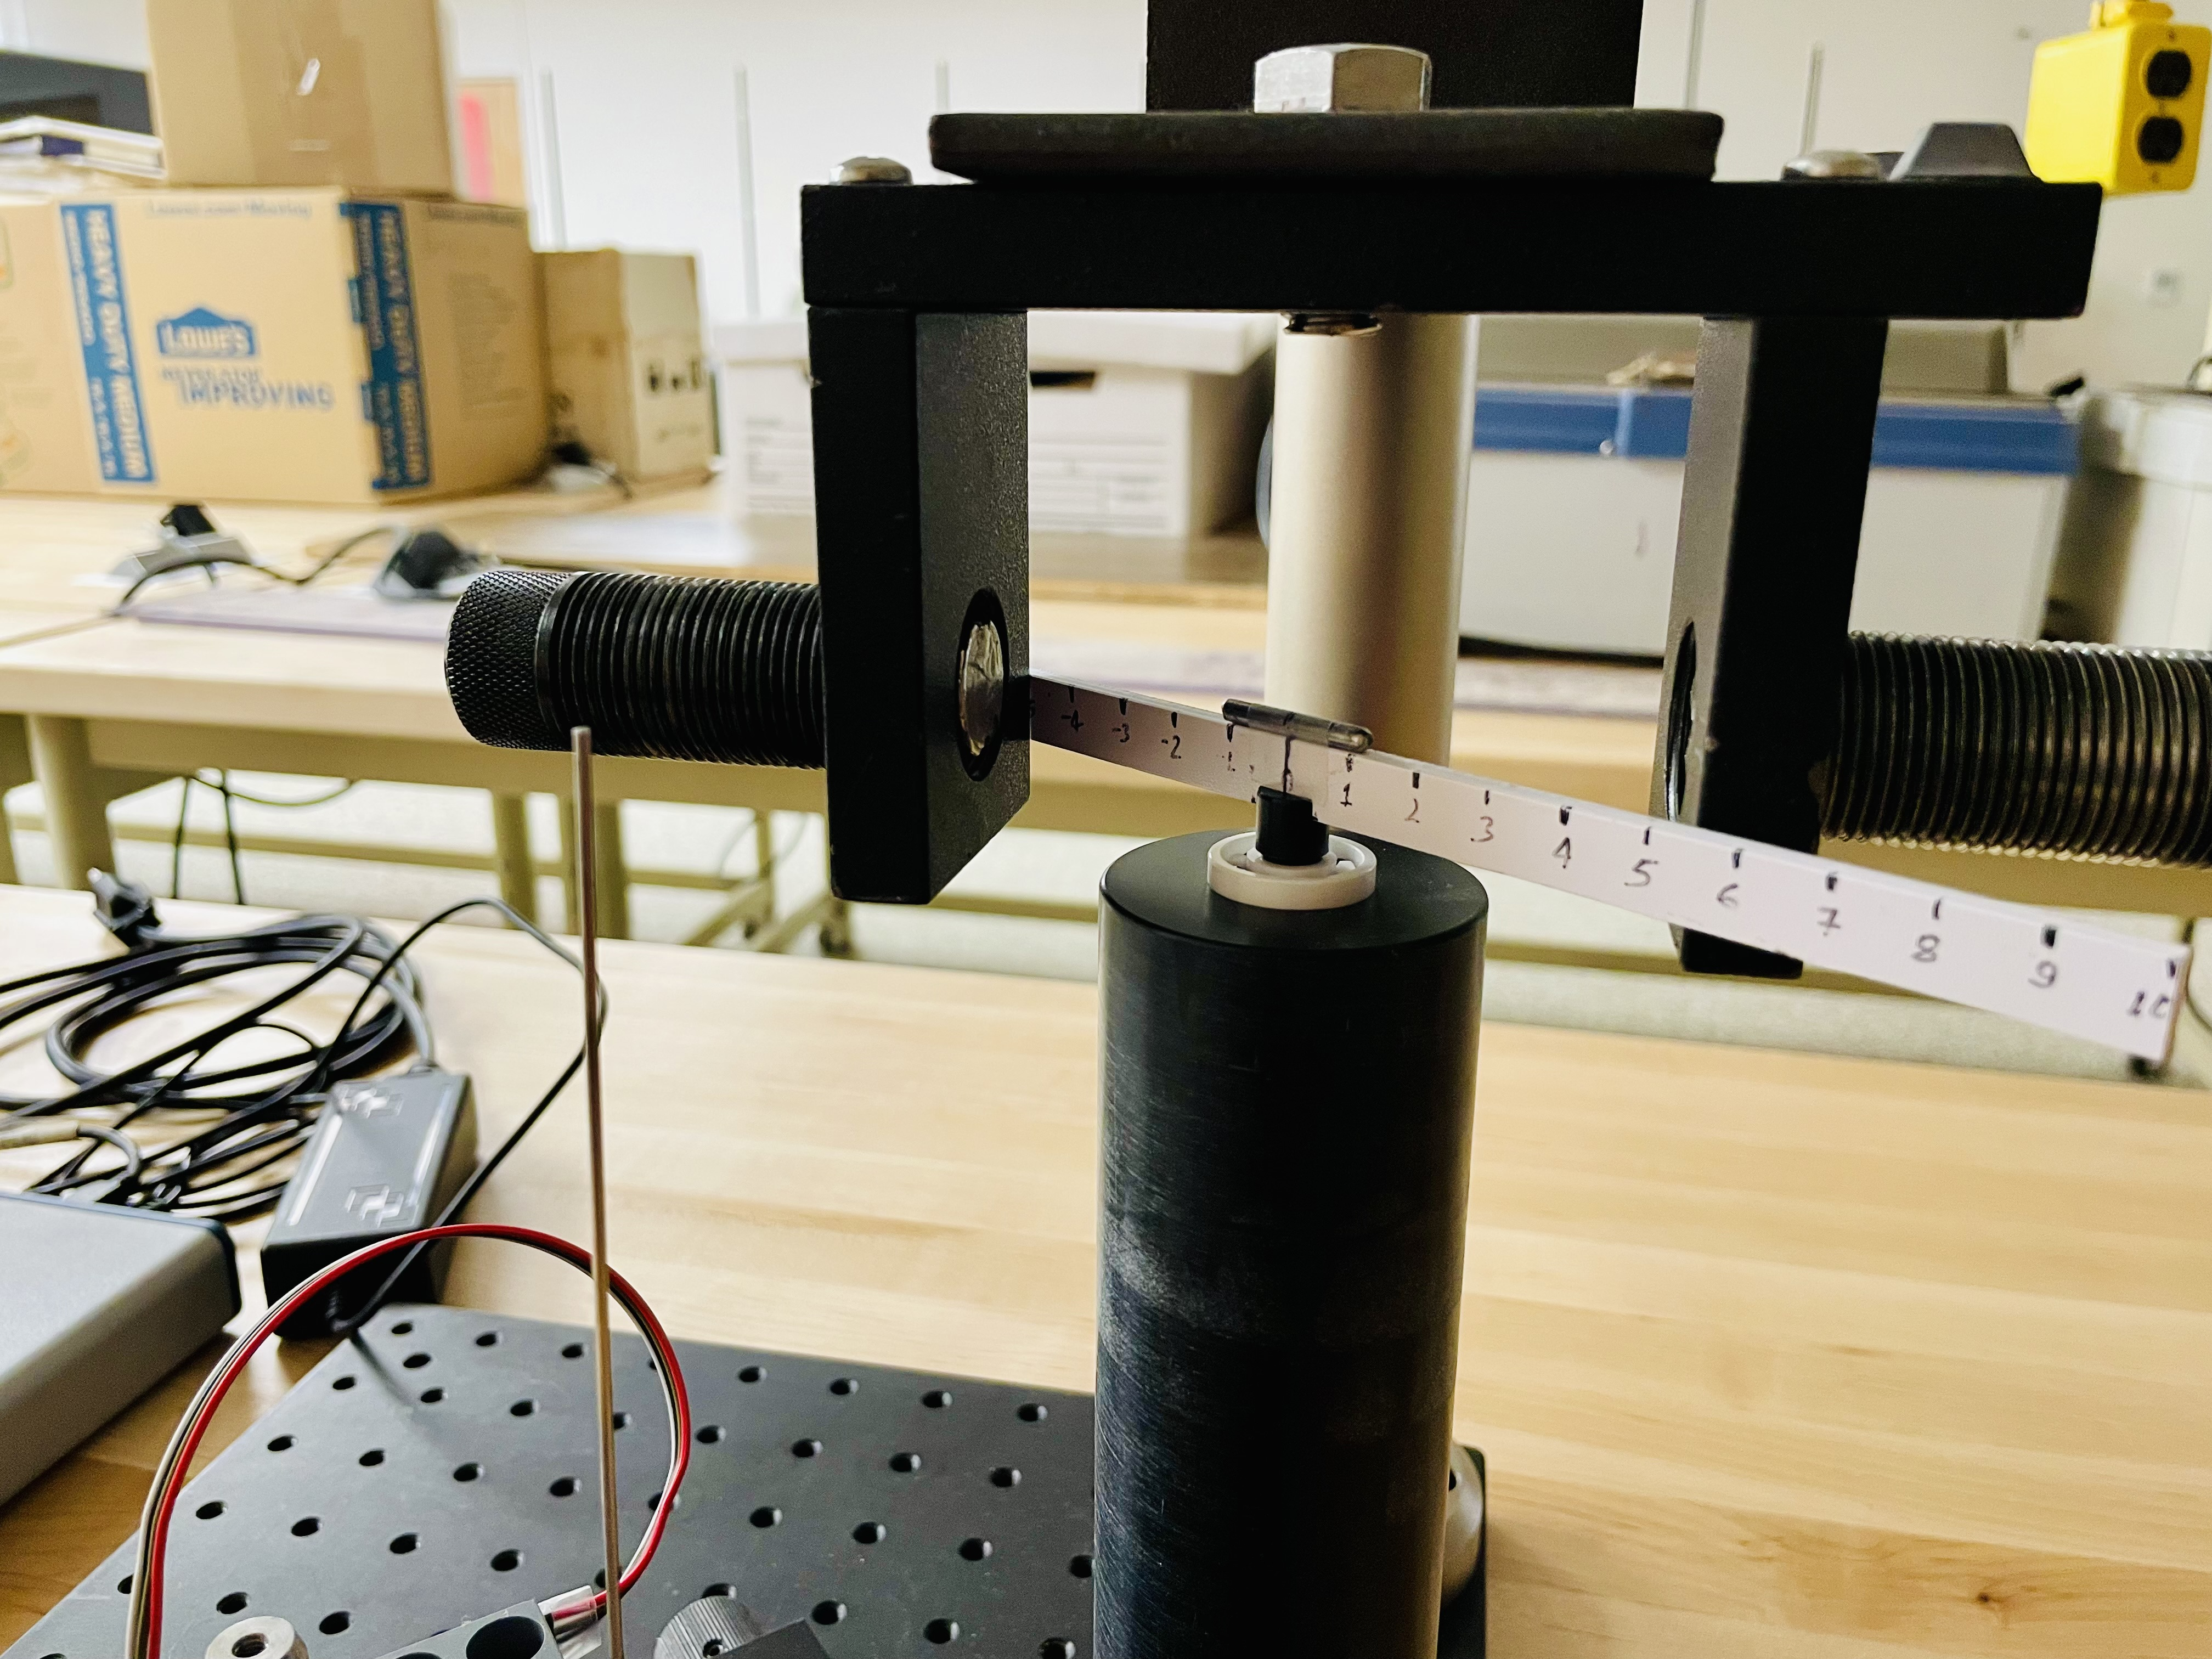
\includegraphics[width=\textwidth]{Assests/torquesCloseup.jpg}
		\subcaption{Close up to the neodymium magnets and test sample (cylindrical metallic piece) were torques are applied.}
	\end{minipage}
	\caption{Implementation of the apparatus in the laboratory setting.}
	\label{fig:torqueDevice}
\end{figure}



%\input{chapter3}

%\input{chapter4}

%\input{chapter5}
%\clearpage

\appendix %begin appendix section
%\chapter{Style guide} \label{sec:appa}% Input Appendix titles as chapters.  \label{sec:appa} is a section label, which makes it easy to reference the section with the command \ref{sec:appa}
%\input{appendixa}
%\clearpage

\chapter{Engineering Drawings} \label{sec:appa}
\includepdf[
pages=1,
landscape=true,
scale=0.85,
pagecommand={%
	\thispagestyle{plain}%
    % Title across the top (in landscape coordinates)
\makebox[0pt][l]{%
	\raisebox{-20cm}[0pt][0pt]{%
		\hspace*{-2cm}%
		\rotatebox{90}{\Huge\textbf{Appendix A: Engineering Drawings}}%
	}%
}
	\makebox[0pt][l]{%
		\raisebox{2cm}[0pt][0pt]{\hspace*{2cm}\Huge\textbf{Appendix A1: Pole drawing}}%
	}%
}
]{Assests/schematic.pdf}



\includepdf[
pages=-,
landscape=true,
scale=0.85,
pagecommand={%
	\thispagestyle{plain}%
	\makebox[0pt][l]{%
		\raisebox{2cm}[0pt][0pt]{\hspace*{2cm}\Huge\textbf{Appendix A2: Frame drawing}}%
	}%
}
]{Assests/Planos_marco.pdf}


\chapter{Calibrations} \label{sec:appb}
\renewcommand{\thefigure}{B.\arabic{figure}}
\setcounter{figure}{0}

\section*{Appendix B: Calibration Logs and Supplementary Graphs}

Additional experimental relationships and fitting diagnostics are presented to support the main analysis.

\begin{figure}[H]
	\centering
	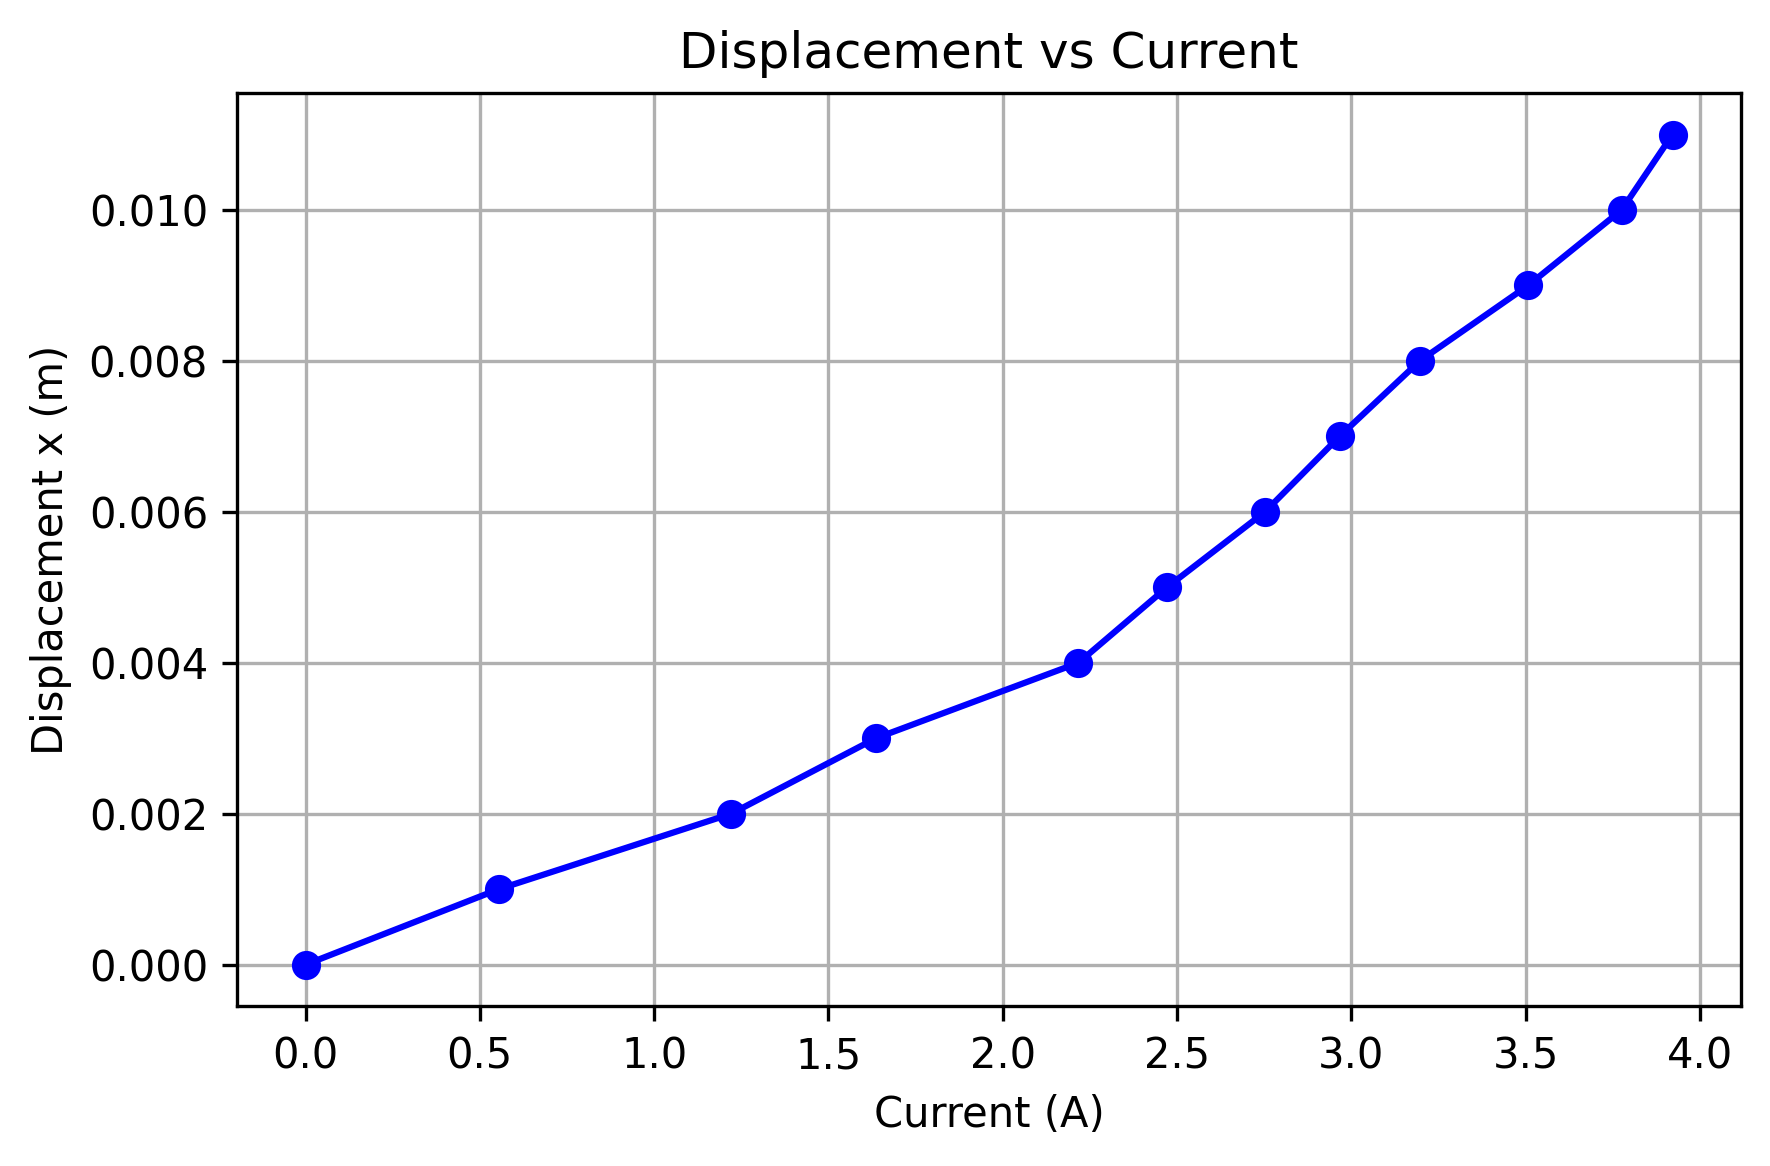
\includegraphics[width=0.85\textwidth]{Assests/Displacement_vs_Current.png}
	\caption{Displacement as a function of current through the solenoid.}
\end{figure}

\begin{figure}[H]
	\centering
	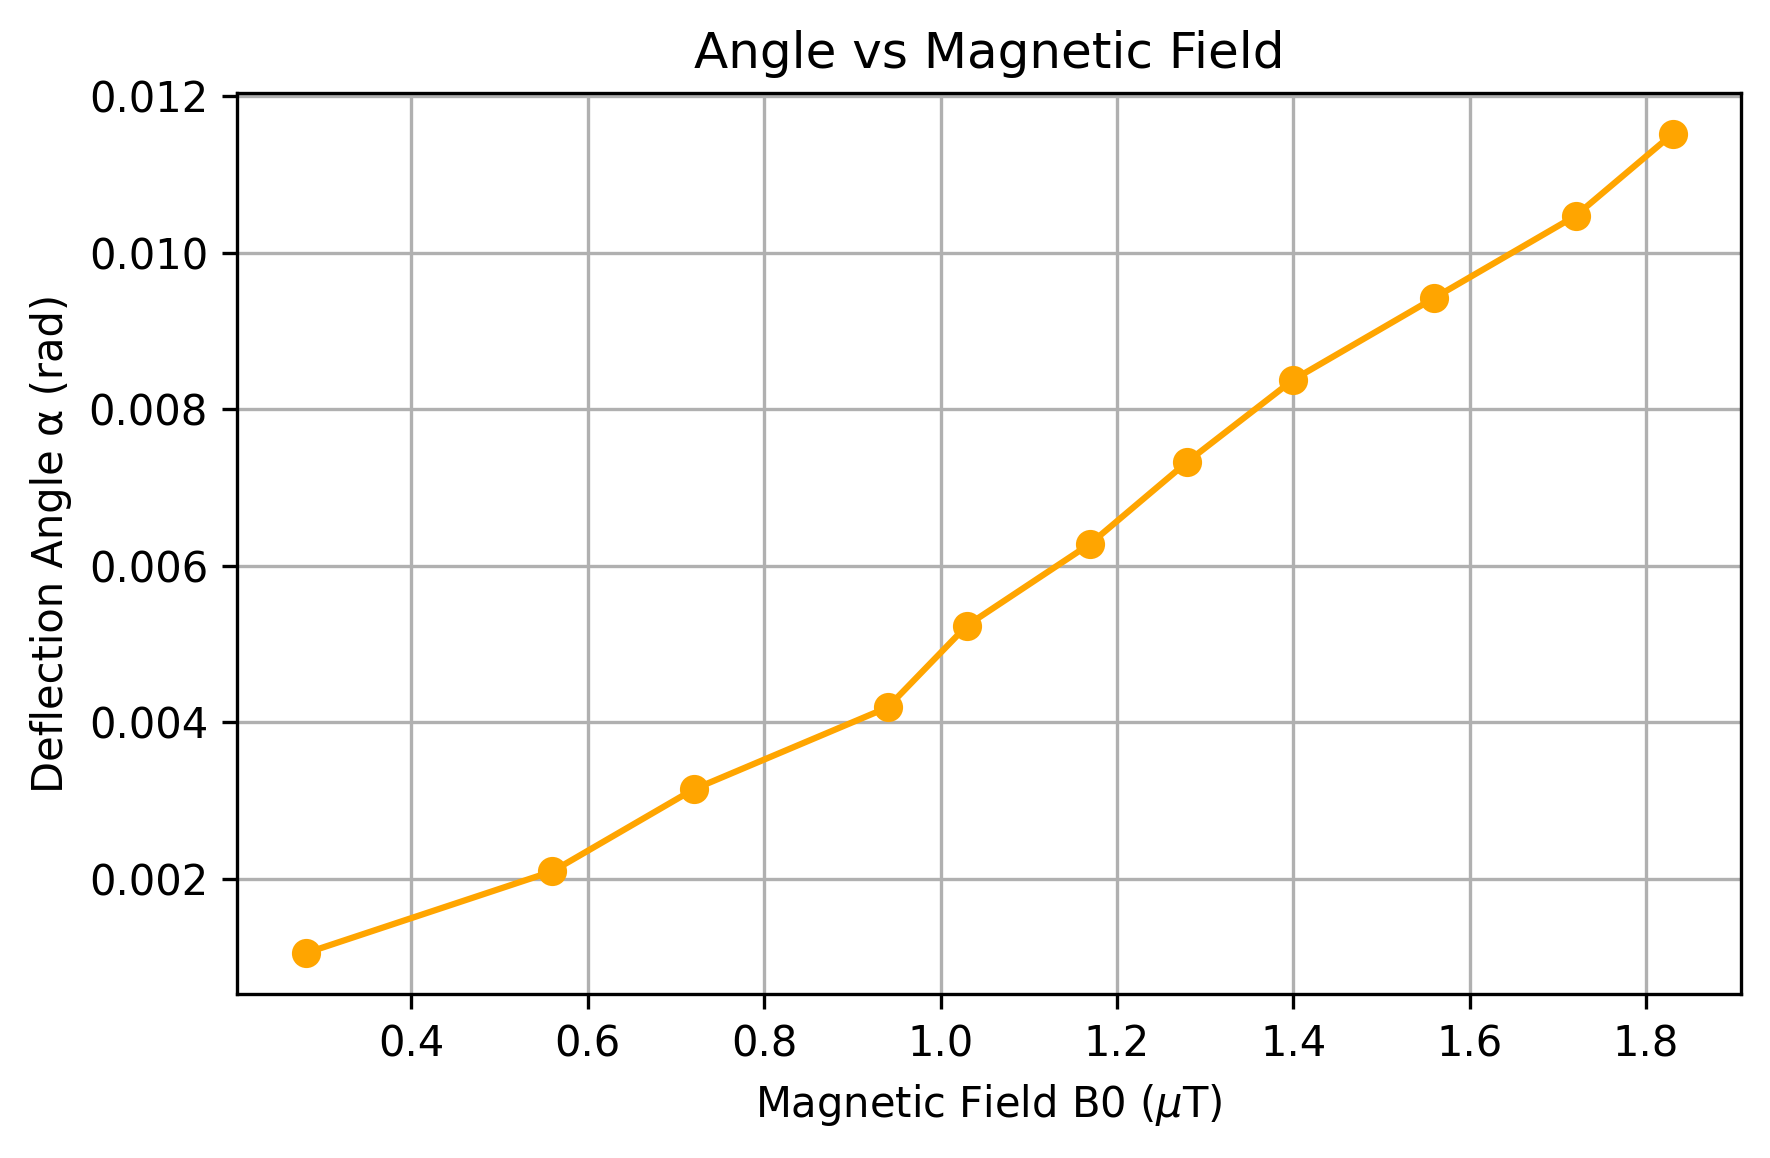
\includegraphics[width=0.85\textwidth]{Assests/Angle_vs_Field.png}
	\caption{Measured angle $\alpha$ versus magnetic field intensity $B_0$.}
\end{figure}

\begin{figure}[H]
	\centering
	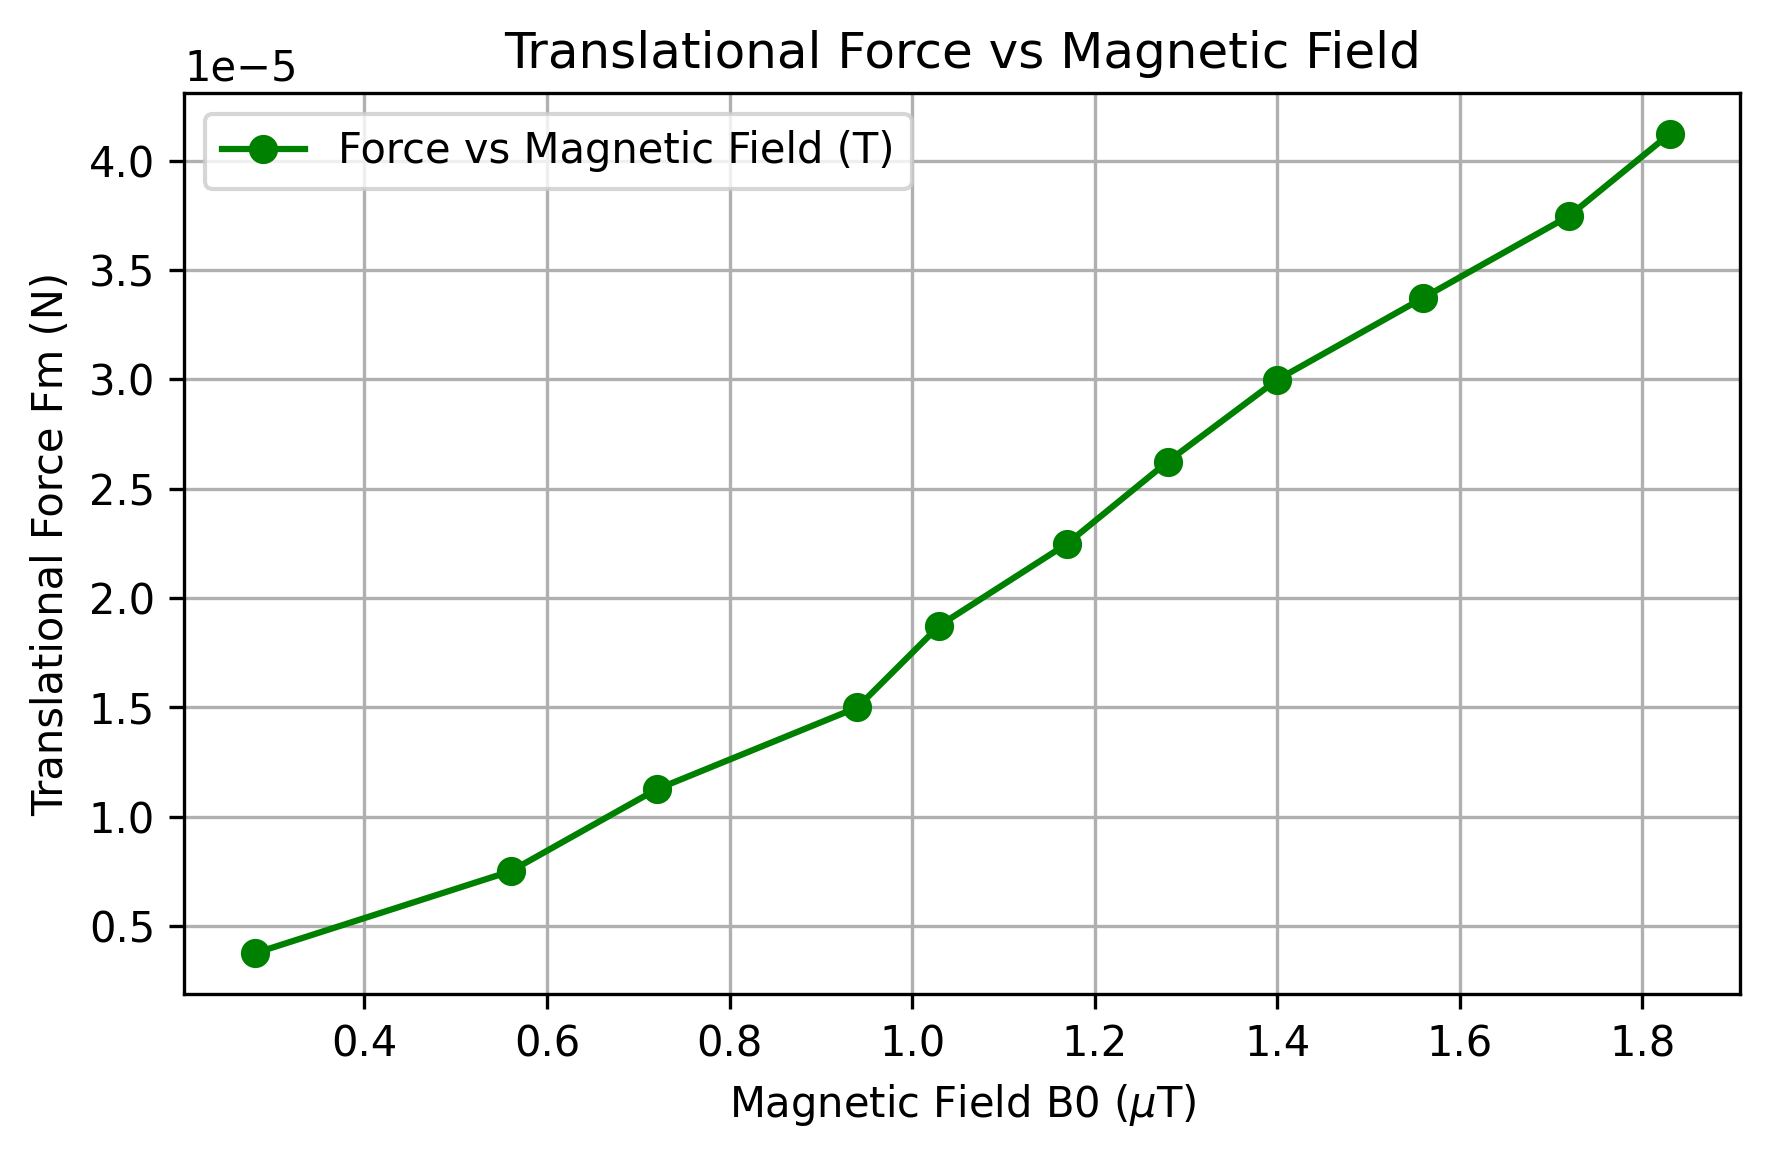
\includegraphics[width=0.85\textwidth]{Assests/Force_vs_Field.png}
	\caption{Computed translational force $F_m$ as a function of $B_0$.}
\end{figure}

\begin{figure}[H]
	\centering
	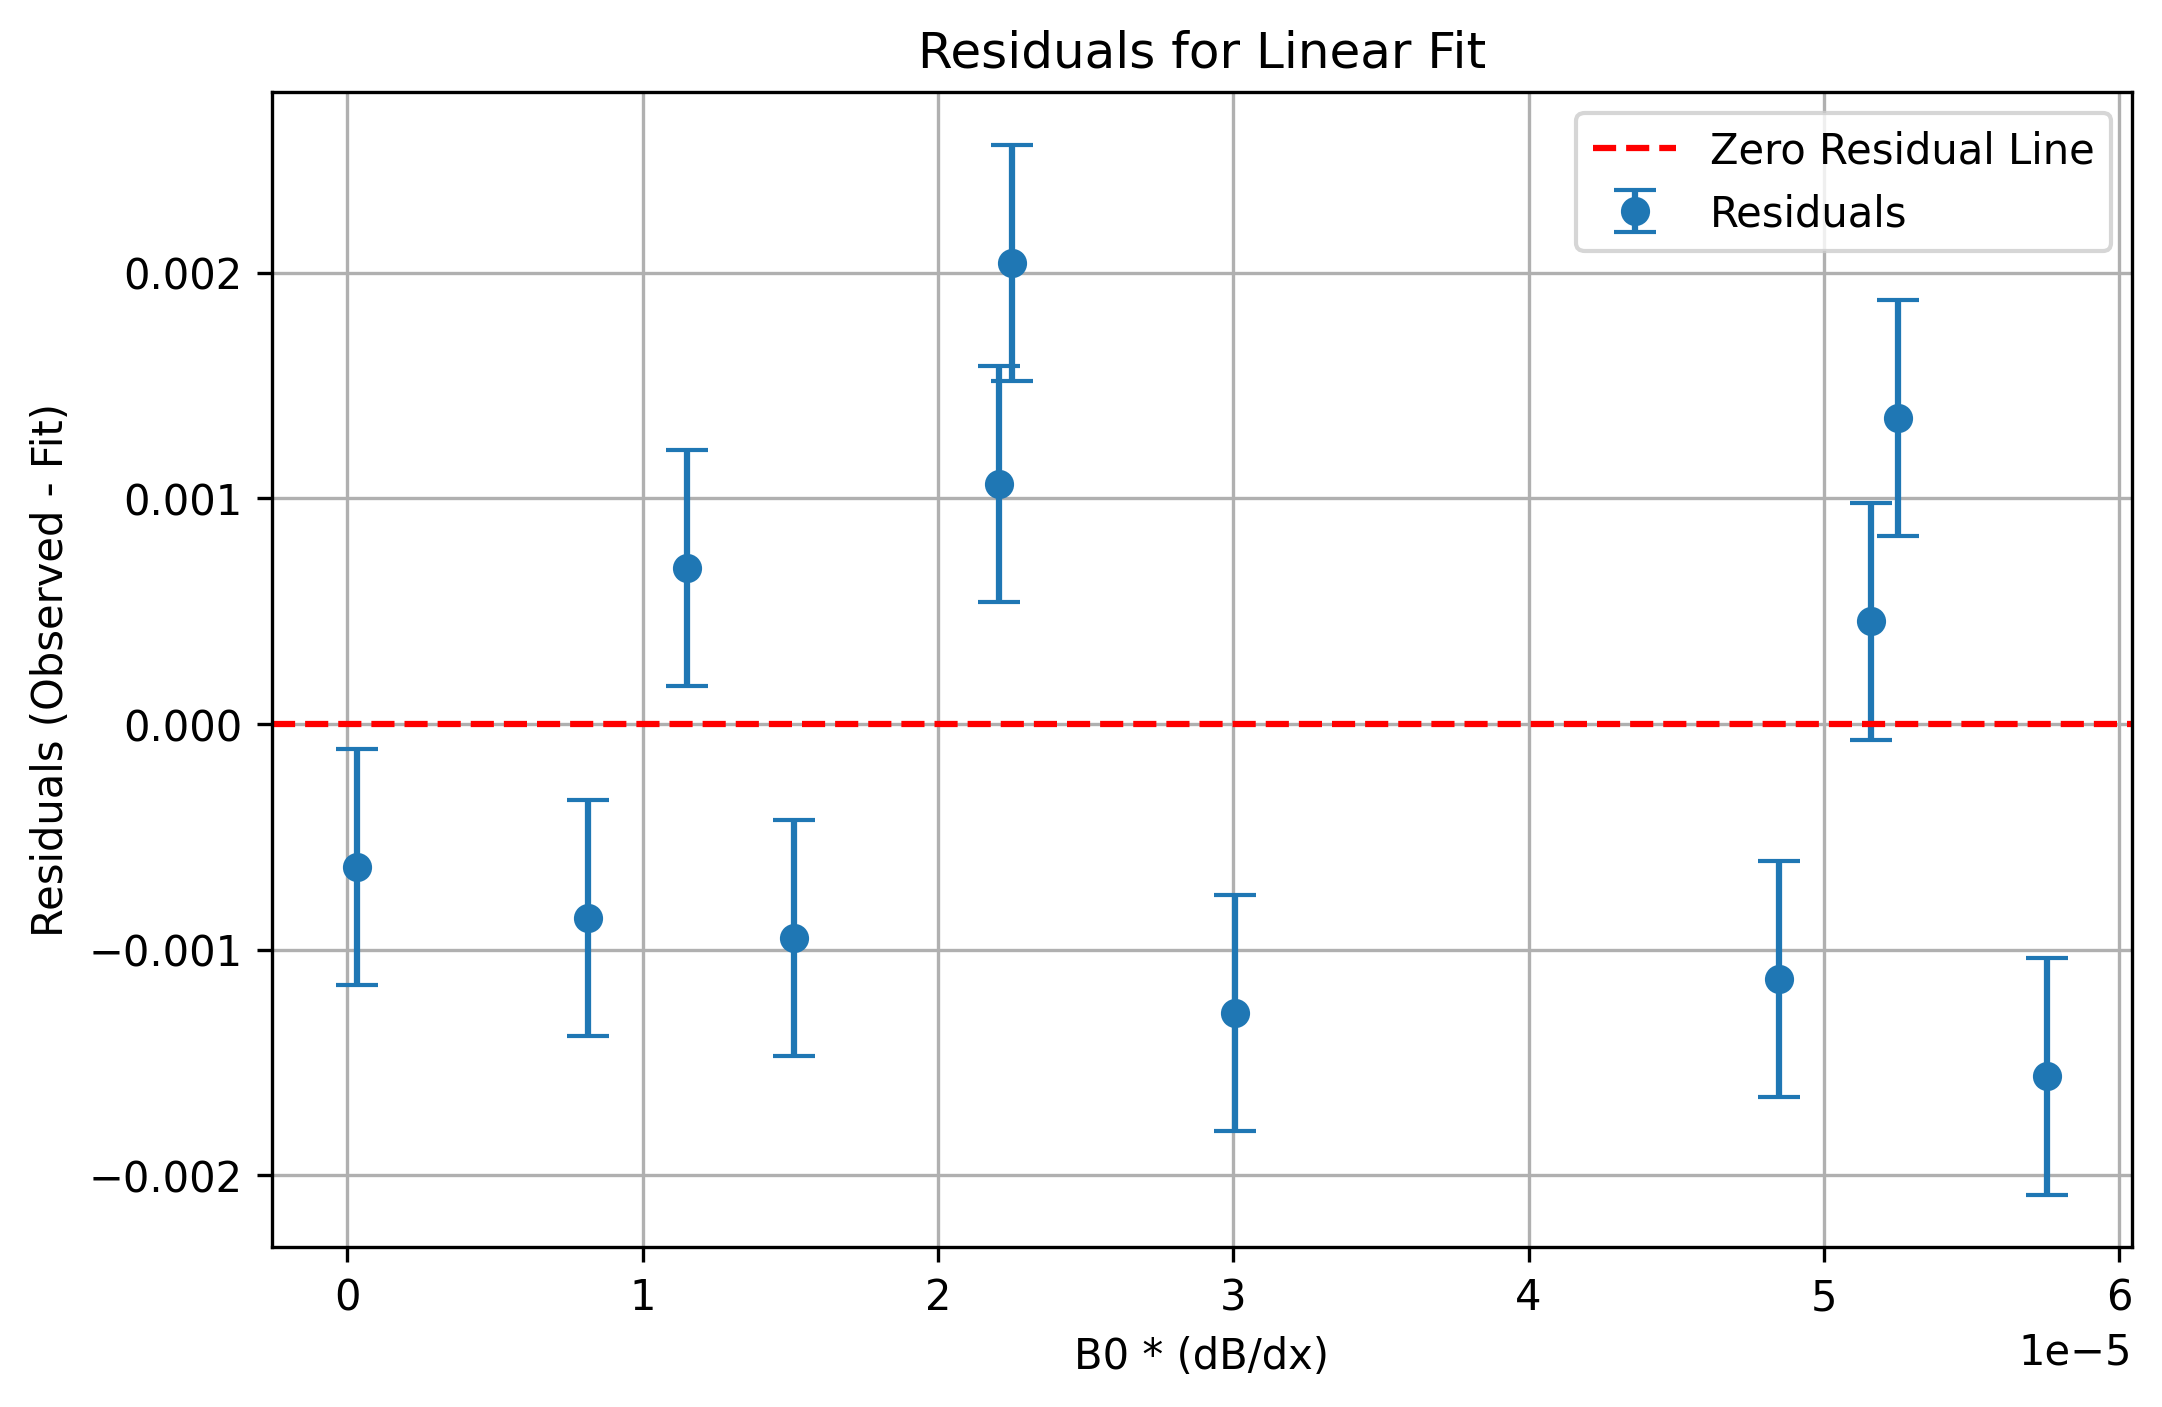
\includegraphics[width=0.85\textwidth]{Assests/Residuals_Plot.png}
	\caption{Residuals from linear fit of $\tan(\alpha)$ vs. $B_0 \cdot \frac{dB_0}{dz}$. Error bars indicate propagated uncertainties.}
\end{figure}

\begin{figure}[H]
	\centering
	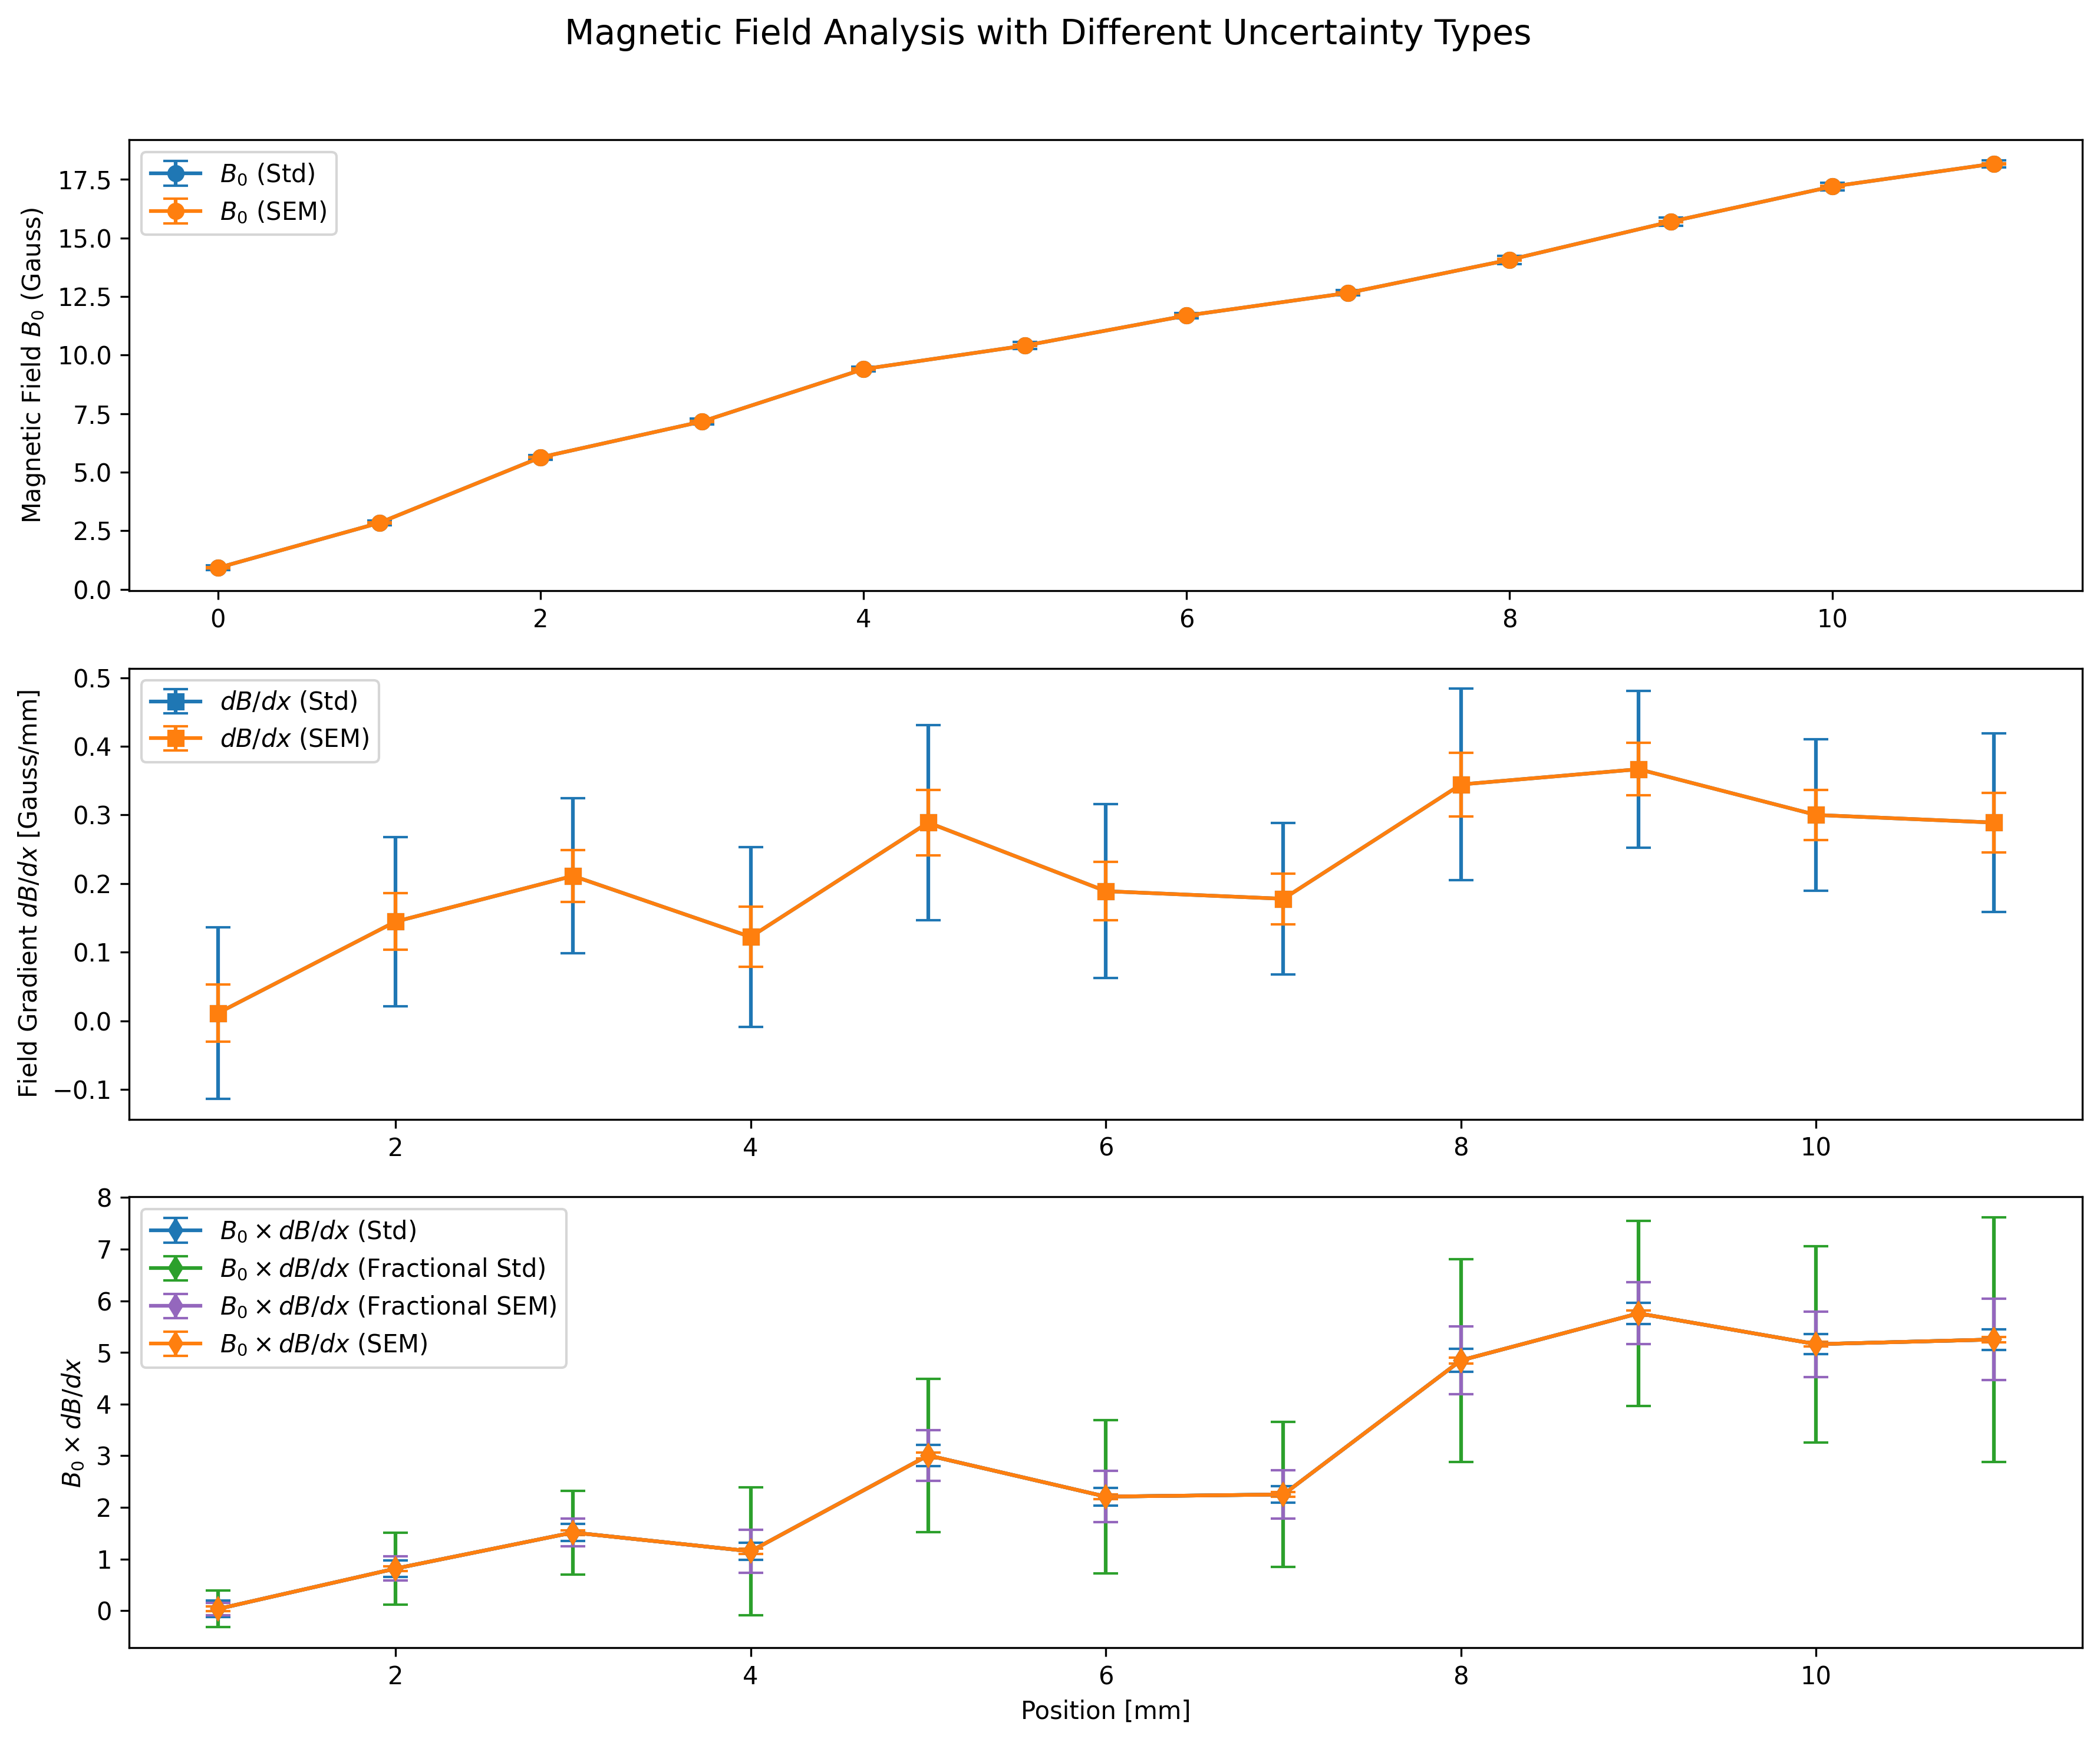
\includegraphics[width=\textwidth]{Assests/Uncertainty_Propagation_Plot.png}
	\caption{Propagation of measurement uncertainty through magnetic field analysis. Top: Measured field $B_0$ with standard deviation and SEM. Middle: Gradient $dB/dz$ with propagated error. Bottom: Final product $B_0 \cdot dB/dz$ with multiple uncertainty estimations (standard, fractional, SEM). This term was used as the independent variable in the susceptibility fit.}
	\label{fig:uncertainty}
\end{figure}


\chapter{Copyright permissions}\label{sec:appc}
Unless you substantially alter a figure, you are not allowed to use figures from a published document, including journal articles, without copyright permission from the publisher.  This is usually easily secured, without cost to you.  Go to the journal article or book on the publisher's website, and find the Copyrights/Permissions link.  Just fill out the form or follow instructions, and you will be emailed documentation of permission to use the figure in your thesis.  For more information on using copyrighted figures in your thesis, see 

\href{http://guides.lib.umich.edu/dissertationcopyright/otherscontent}{http://guides.lib.umich.edu/dissertationcopyright/otherscontent}.

You can include the copyright permissions in an appendix as figures or include a pdf using this command \verb!\includepdf[scale=0.9]{rsna.pdf}!. If you do this, you could reference the appendix in each figure caption with ``(See Appendix B for documentation of permission to republish from [cite source].)" Alternatively, you can save your permission documents into a separate document and include them as a separate upload to the \gls{cdr}.  Make sure you note in your thesis that you are using the figure with permission.  Please talk to Richard Jizba at the Creighton Library for advice.  



%\clearpage



\addcontentsline{toc}{chapter}{Glossary}
\printnoidxglossaries

%\clearpage

%.tex method to make a references section
%\addcontentsline{toc}{chapter}{References}
%\input{biblio}

%.bib method for a references section
\bibliography{references}
%\bibliographystyle{IEEEtran}
\bibliographystyle{unsrt}




\end{document}